\documentclass{article}
\usepackage{graphicx} % Required for inserting images
\usepackage{biblatex}
\usepackage{xcolor}
\usepackage{physics}
\addbibresource{refs.bib}
\usepackage{geometry}
\usepackage{subcaption}


\RequirePackage{xcolor}
\newcommand{\revision}[1]{{\color{red}{#1}}}
\newcommand{\ts}[1]{{\color{red}- \textbf{Thiago}: #1 - }}
\newcommand{\ca}[1]{{\color{orange} - \textbf{Cesar}: #1 - }}

\geometry{
    left=15mm,
    right=15mm,
    top=15mm,
    bottom=15mm
}
\usepackage{amsmath}
\usepackage{amssymb}

\title{Open Jaynes-Cummings Model with Time-dependent Light-Matter Coupling}
\author{Cesar Amaral, Thiago T. Tsutsui}
\date{September 2025}

\begin{document}

\maketitle

\section{Introduction}
In this work, we consider two simultaneous generalizations of the Jaynes-Cummings (JC) model: the open extension \cite{Barnett1986,Puri1988} and the time-dependent extension \cite{Schlicher1989,DeCastro2023}.
In the case of dissipation, 
the effects of decoherence on informational measures has been studied in Ref. \cite{Mohamed2025}, in a double JC\revision{, two qubits and two cavities, }setup and employing the Millburn equation for obtaining the dynamics with initial
Barut-Girardello coherent states for the cavities.
In Ref. \cite{Mohamed2019} they analyzed the Tavis-Cummings model, but with the intrinsic decoherence model.
In the case of the time-dependent JC, quantum correlations between two qubits interacting with a single cavity were studied (Tavis-Cummings), with the inclusion of atomic motion, modeled with an time-dependent coupling \cite{Abdel-Khalek2016a,Algarni2017}.
An particularly interesting work was realized in Ref. \cite{Rendell2003}, where an initial atom-field Bell state was studied in the case of dephasing. 
Correlations and trace distance in open systems dynamics: \cite{Smirne2010}
Nonclassicality in driven open Jaynes-Cummings model: \cite{Clemens2000}.

Effects of dissipation on Schr\"odinger cat states: \cite{Walls1985,Phoenix1990,Kim1992}

Three dissipations simultaneously and good interpretations: \cite{Auffeves2010}. 
They stablish a different ``good/bad'' cavity regime in the open systems context.

The combined effect of these two generalizations has not been fully explored in the JC literature. 
Importantly, in Ref. \cite{Elliott2024}, Wigner negativity was investigated, with the driven and open JC model, considering cavity and atom decoherence.
However, they considered a constant coupling. 
\ts{Nesse paper do Elliot tem uma frase legal sobre como cavidades modernas permitem acoplamentos fortes.}
In Ref. \cite{Kolar2024}, the interaction between an artificial molecule and an harmonic oscillator was analyzed using the \revision{Bloch-Redfield} master equation, with the objective of investigating how a decaying atom-field coupling could generate superpositions of states with negative Wigner functions.
Therein, the initial state of the system is a \emph{global} thermal state. 
Employing the power-law potentials, Abdel-Khalek and coworkers studied the time-dependent JC with phase-damping in the cavity \cite{Abdel-Khalek2016b}; they computed negativity, atomic inversion, Wehrl entropy and field entropy with a cosine modulation in the coupling to model atomic movement.
%Additionally, Korashy \emph{et al.} \cite{Korashy2021} studied %a five-level atom interacting with a single mode-field %considering a time-dependent coupling, 
%with effects in the phase-space probability distribution. 


\section{Linear coupling}
First, we consider a modulation of the type 
\begin{equation}
    g(t)=g_0\left(\zeta t+w\right).
\end{equation}

\subsection{$g_0=1,\,\zeta=0.2,\,\omega=0, \, \kappa=0.05, \,  \gamma=0, \, \gamma_{\phi_0}=0$}
In this instance, the coupling begins in $g(0)=0$ and evolves to $g(30)=6$,
simulating a fast evolution of the cavity mode.
For $t\leq5$, the time-dependent coupling is smaller than the constant coupling $g_0$.
In Fig. \ref{fig:grid_cavity_1}, we present the results.

(a) For the open system dynamics, we observe an super-Poissonian dominance.
For early times (until a little later than $t=5$), we obtain more non-classicalities in the photon probability distribution.

(b) For open systems and early times, we note more oscillations in the atom populations in the time-dependent regime than in the constant coupling. 
In neither of the cases, there is a full revival.
However, small residual oscillations persist in the ``revival region'' (using the ideal case as a frame of reference), with larger amplitudes in the time-dependent scenario. 

(c) For an specific time interval and cavity dissipation, the time-dependent coupling version of the dynamics possesses more entanglement (measured with negativity) than the constant coupling.
For later times, the entanglement with varying coupling is smaller.
Curiously, in the closed system, the time-dependent coupling leads to generally higher entanglement.

\begin{figure}[t]
    \centering
    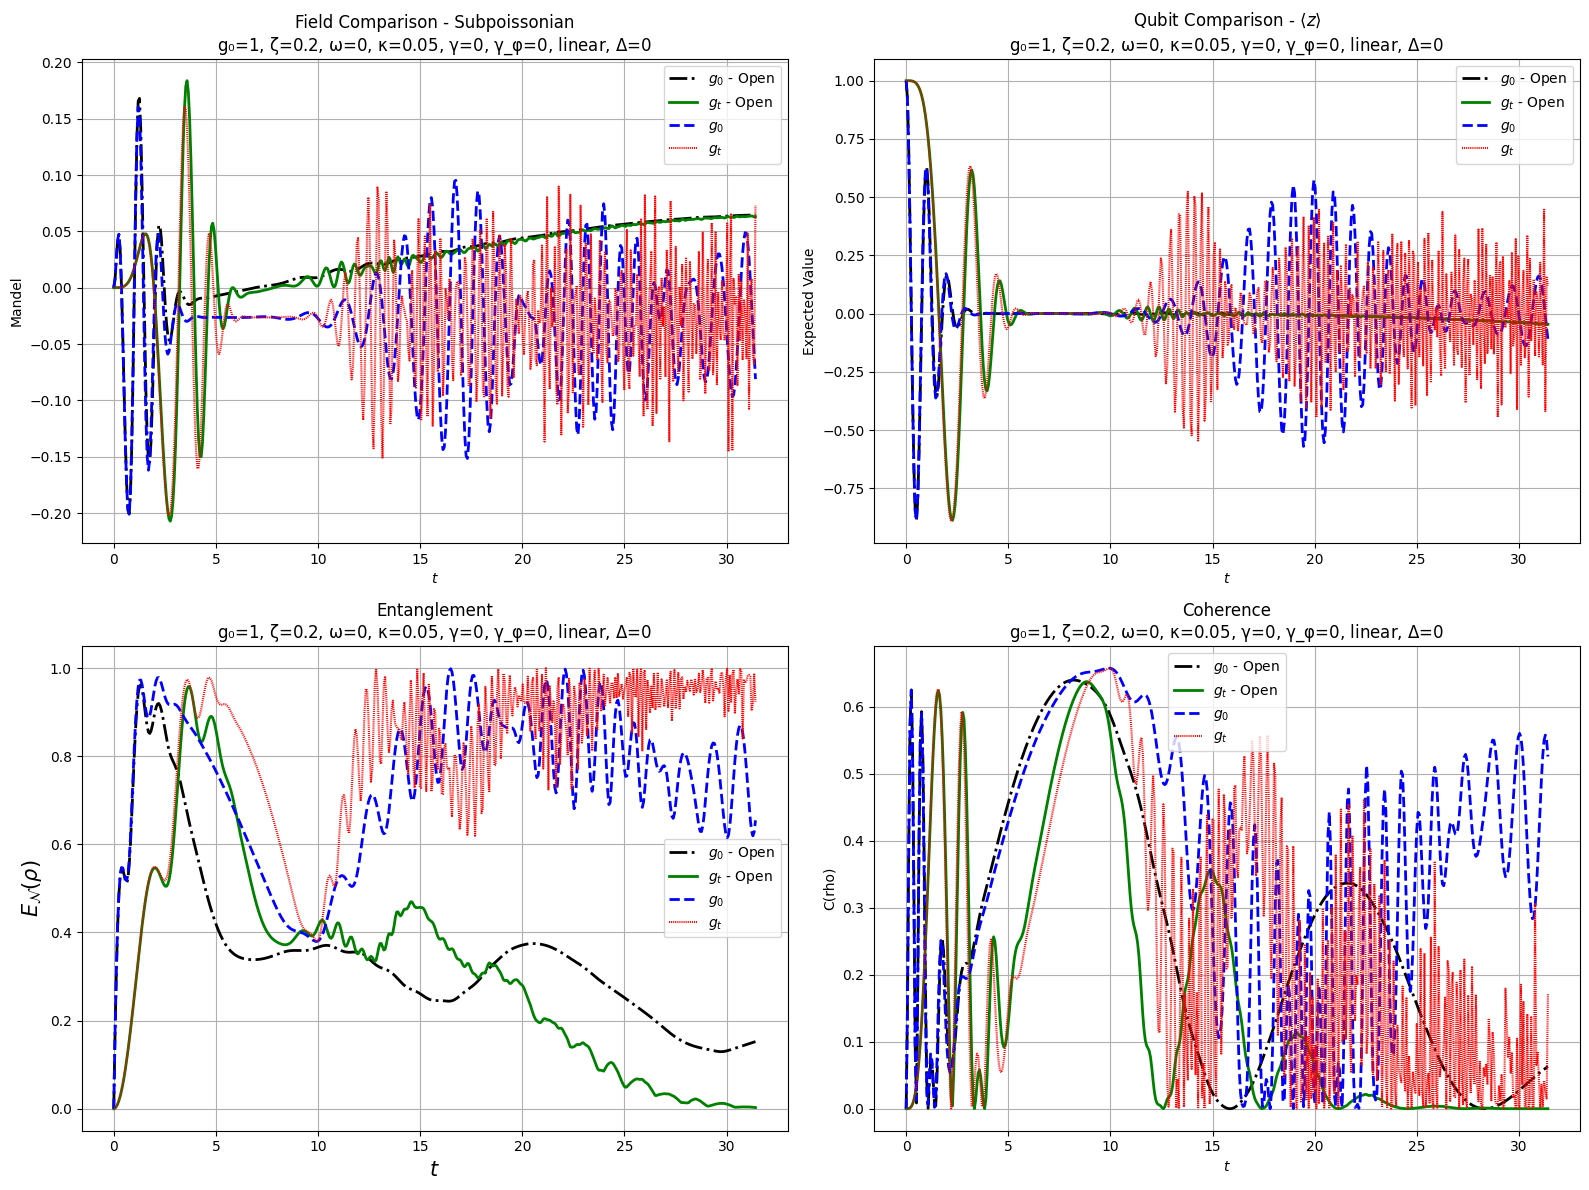
\includegraphics[width=1\linewidth]{images/grid_cavity_1.png}
    \caption{Results for $g_0=1,\,\zeta=0.2,\,\omega=0, \, \kappa=0.05, \,  \gamma=0, \, \gamma_{\phi_0}=0$.}
    \label{fig:grid_cavity_1}
\end{figure}

\subsection{$g_0=1,\,\zeta=0.01,\,\omega=0, \, \kappa=0.05, \,  \gamma=0, \, \gamma_{\phi_0}=0$}
In this instance, the coupling begins in $g(0)=0$ and evolves to $g(30)=0.3$.
Thus, it simulates an adiabatic evolution of the cavity mode. 
Results in Fig. \ref{fig:grid_cavity_2}.

(a) For the time-dependent open case, we obtain interesting oscillations between super and sub-Poissonian, characteristic of the slow evolution.
We have a bigger peak in sub-Poissonian statistics for the time-dependent open case.

(b) Effects of a slower start in the qubit populations.

\begin{figure}[t]
    \centering
    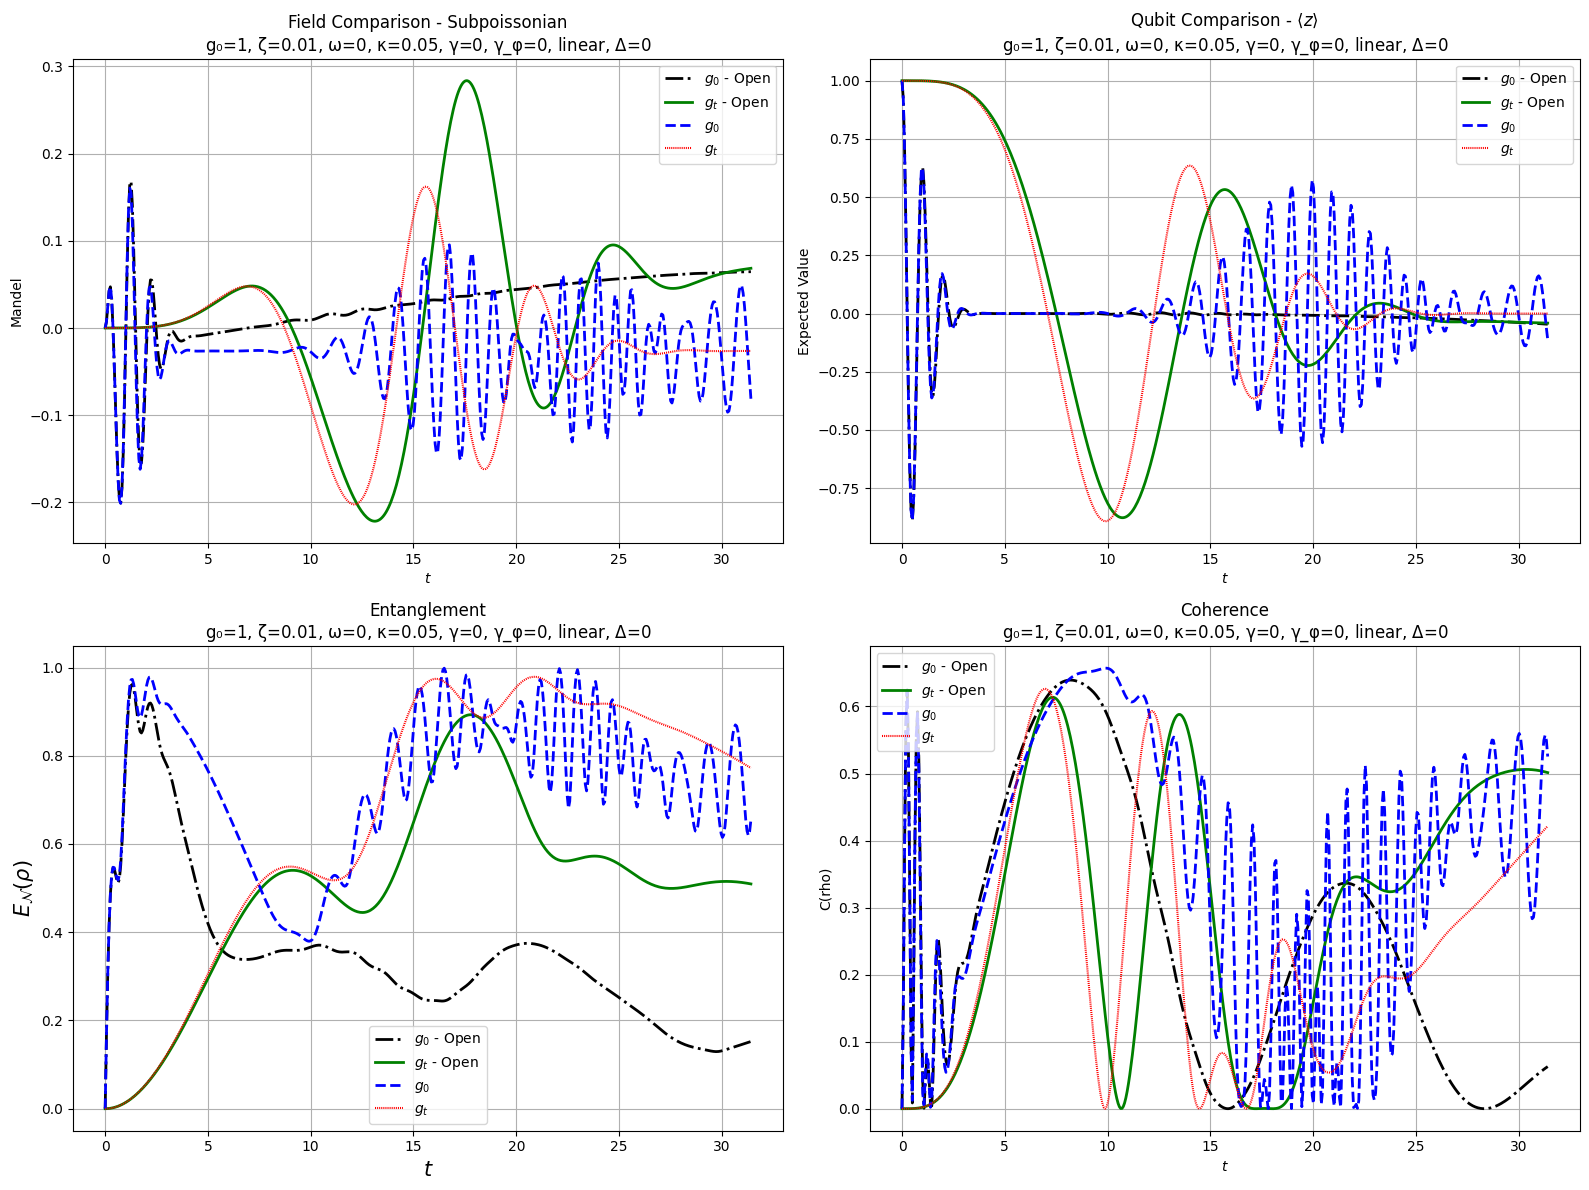
\includegraphics[width=1\linewidth]{images/grid_cavity_2.png}
    \caption{Results for $g_0=1,\,\zeta=0.01,\,\omega=0, \, \kappa=0.05, \,  \gamma=0, \, \gamma_{\phi_0}=0$.}
    \label{fig:grid_cavity_2}
\end{figure}

\subsection{$g_0=1,\,\zeta=0.2,\,\omega=1, \, \kappa=0.05, \,  \gamma=0, \, \gamma_{\phi_0}=0$}
In this instance, the coupling begins in $g(0)=1$ and evolves to $g(30)=7$,
simulating a fast evolution of the cavity mode with non-null initial coupling.
The plots are in Fig. \ref{fig:grid_cavity_3}.
The faster evolution results in a slower decay.
The coupling dictates the interaction with the cavity, which dissipates, resulting in a faster decay of the whole system and of the qubit coherence.

\begin{figure}[t]
    \centering
    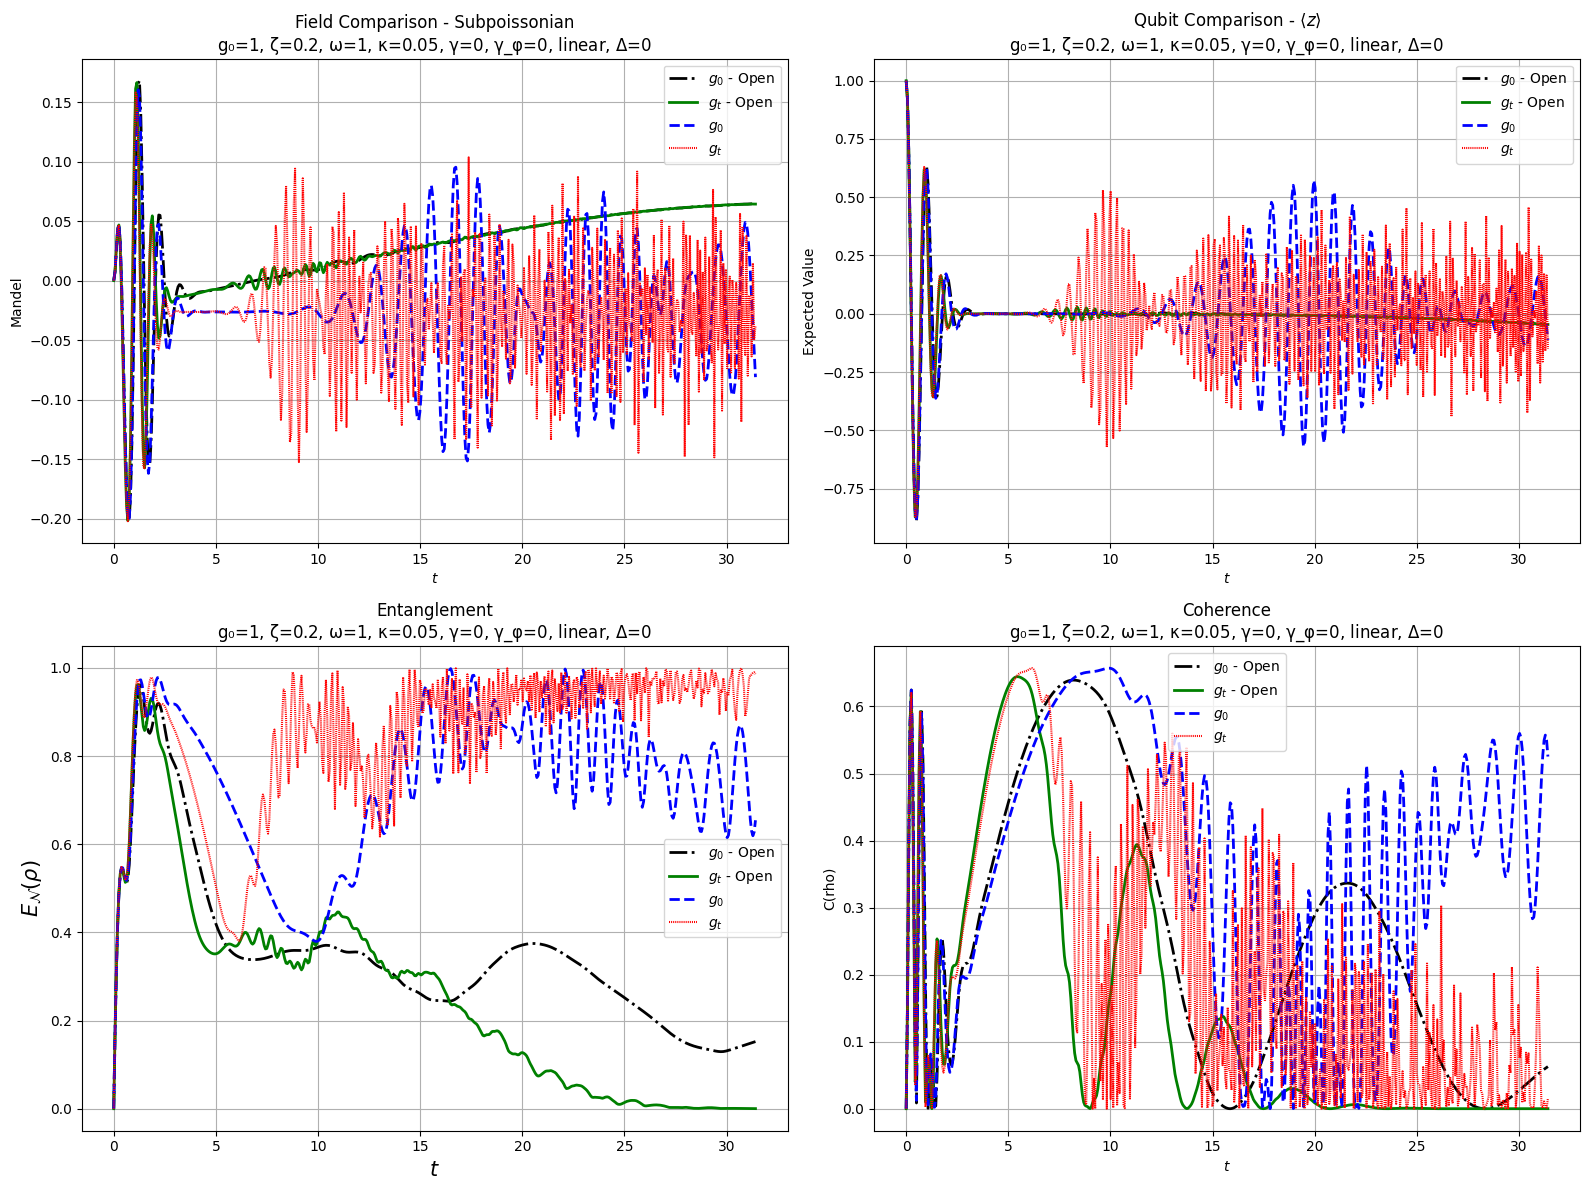
\includegraphics[width=1\linewidth]{images/grid_cavity_3.png}
    \caption{Results for $g_0=1,\,\zeta=0.2,\,\omega=1, \, \kappa=0.05, \,  \gamma=0, \, \gamma_{\phi_0}=0$.}
    \label{fig:grid_cavity_3}
\end{figure}

\subsection{$g_0=1,\,\zeta=0.2,\,\omega=0, \, \kappa=0.05, \,  \gamma=0, \, \gamma_{\phi_0}=0, \, \Delta=0.5,\,  \Delta=1.0$}
In this instance, the detuning affects the oscillations, with a ``trapping effect''. 
The time-dependent versions are more affected.
Refs. \ref{fig:grid_cavity_4} and \ref{fig:grid_cavity_5}.

\begin{figure}[t]
    \centering
    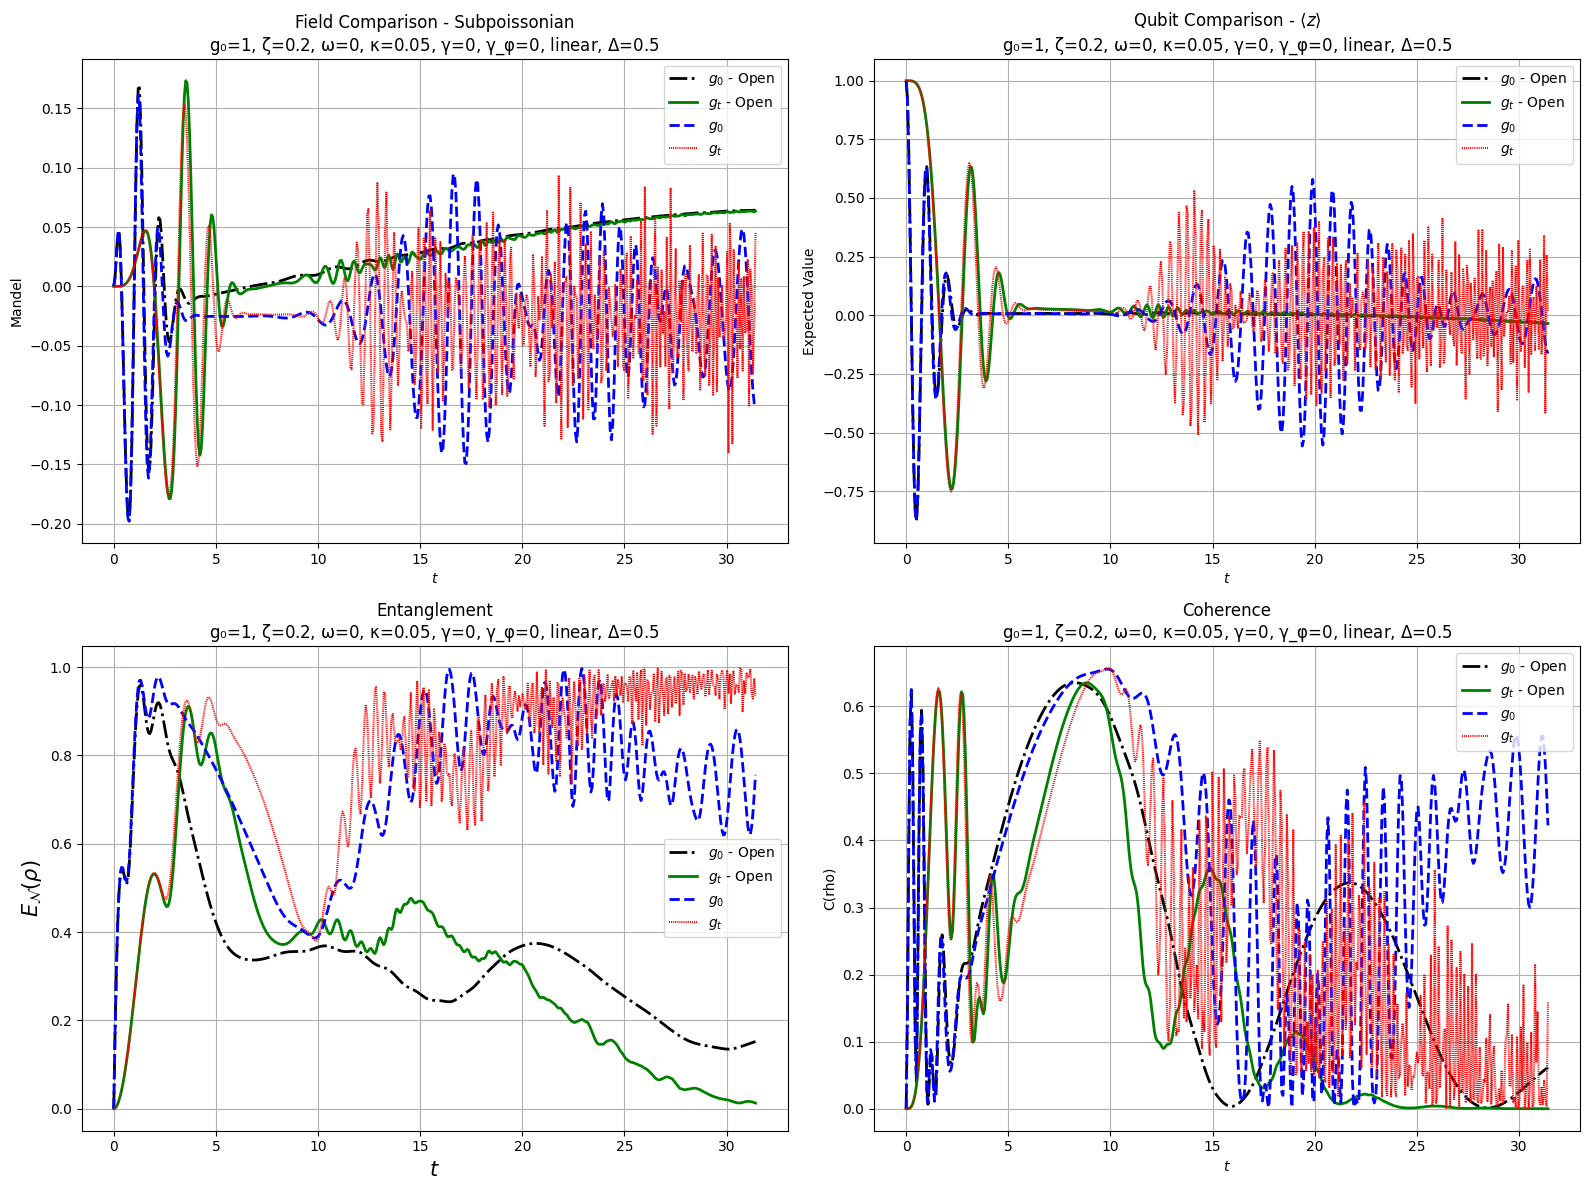
\includegraphics[width=1\linewidth]{images/grid_cavity_4.png}
    \caption{Results for $g_0=1,\,\zeta=0.2,\,\omega=0, \, \kappa=0.05, \,  \gamma=0, \, \gamma_{\phi_0}=0,\, \Delta=0.5$.}
    \label{fig:grid_cavity_4}
\end{figure}

\begin{figure}[t]
    \centering
    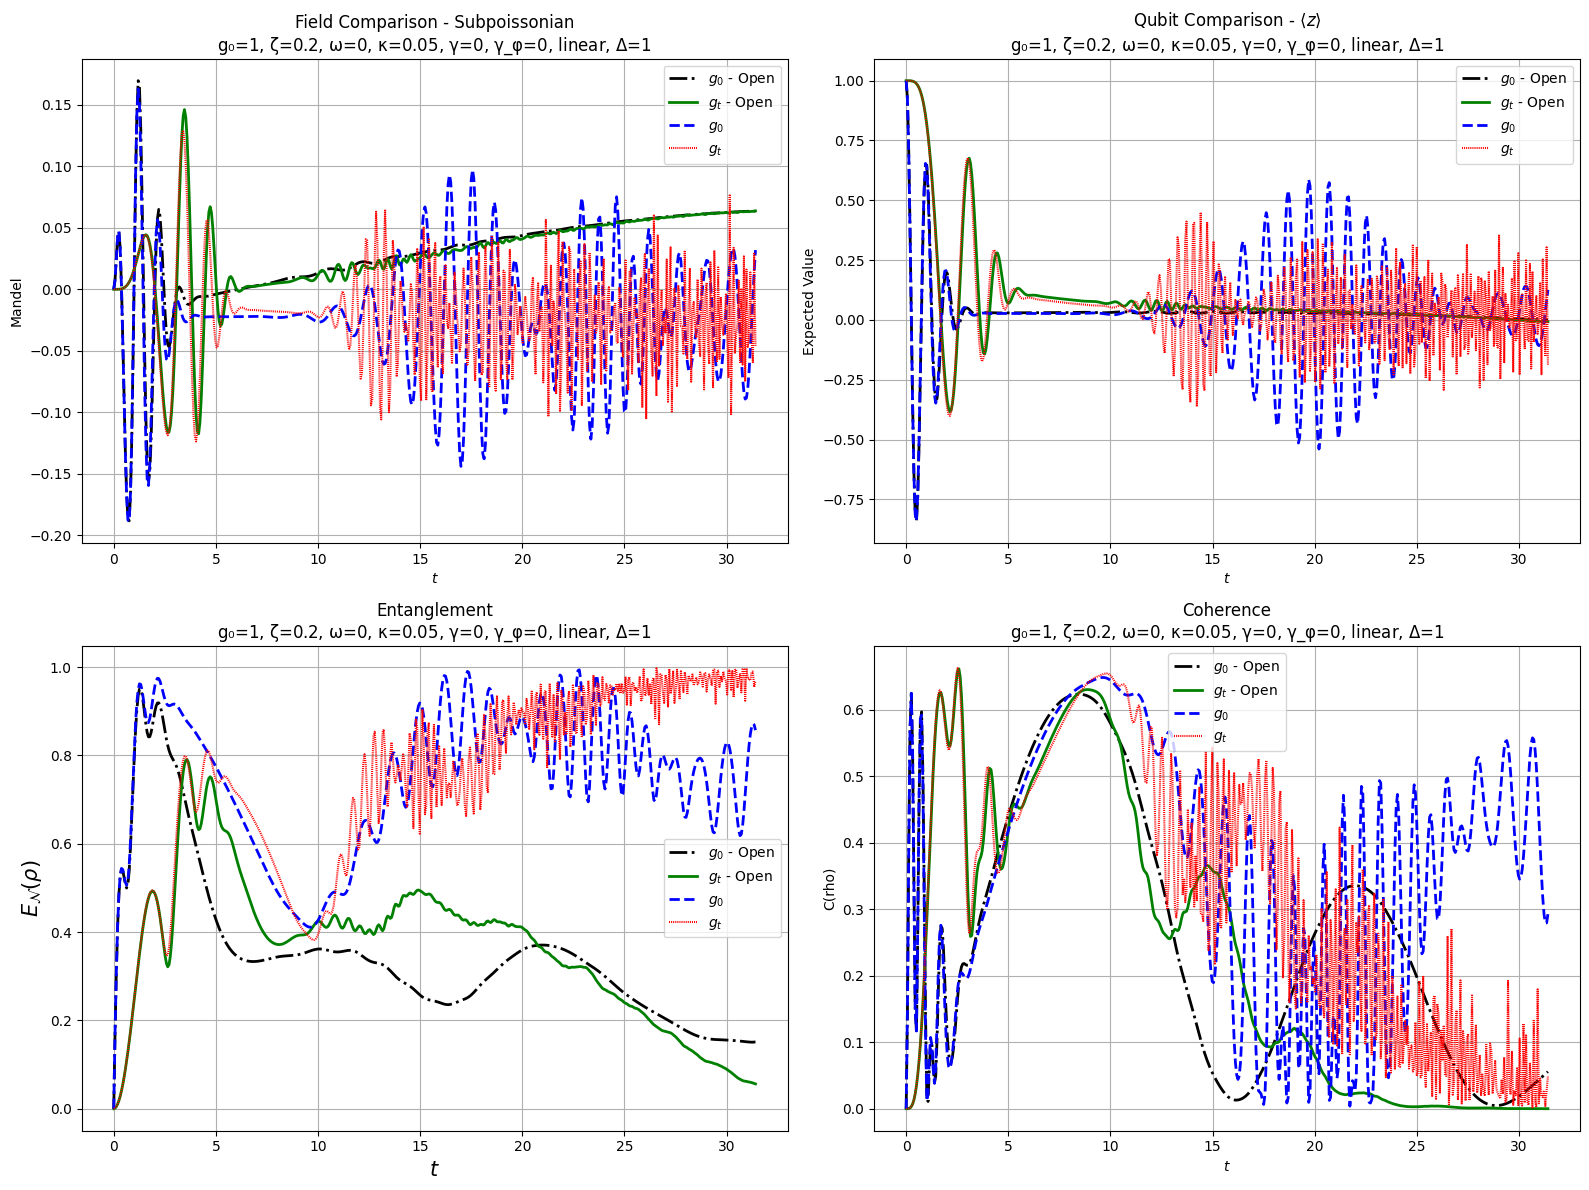
\includegraphics[width=1\linewidth]{images/grid_cavity_5.png}
    \caption{Results for $g_0=1,\,\zeta=0.2,\,\omega=0, \, \kappa=0.05, \,  \gamma=0, \, \gamma_{\phi_0}=0, \, \Delta=1.0$.}
    \label{fig:grid_cavity_5}
\end{figure}

\subsection{$g_0=1,\,\zeta=0.2,\,\omega=0, \, \kappa=0.1, \,  \gamma=0, \, \gamma_{\phi_0}=0, \, \Delta=0$}
The appearance of sub-Poissonian statistic for larger times is strange.
I think there is some numerical error.

\begin{figure}[t]
    \centering
    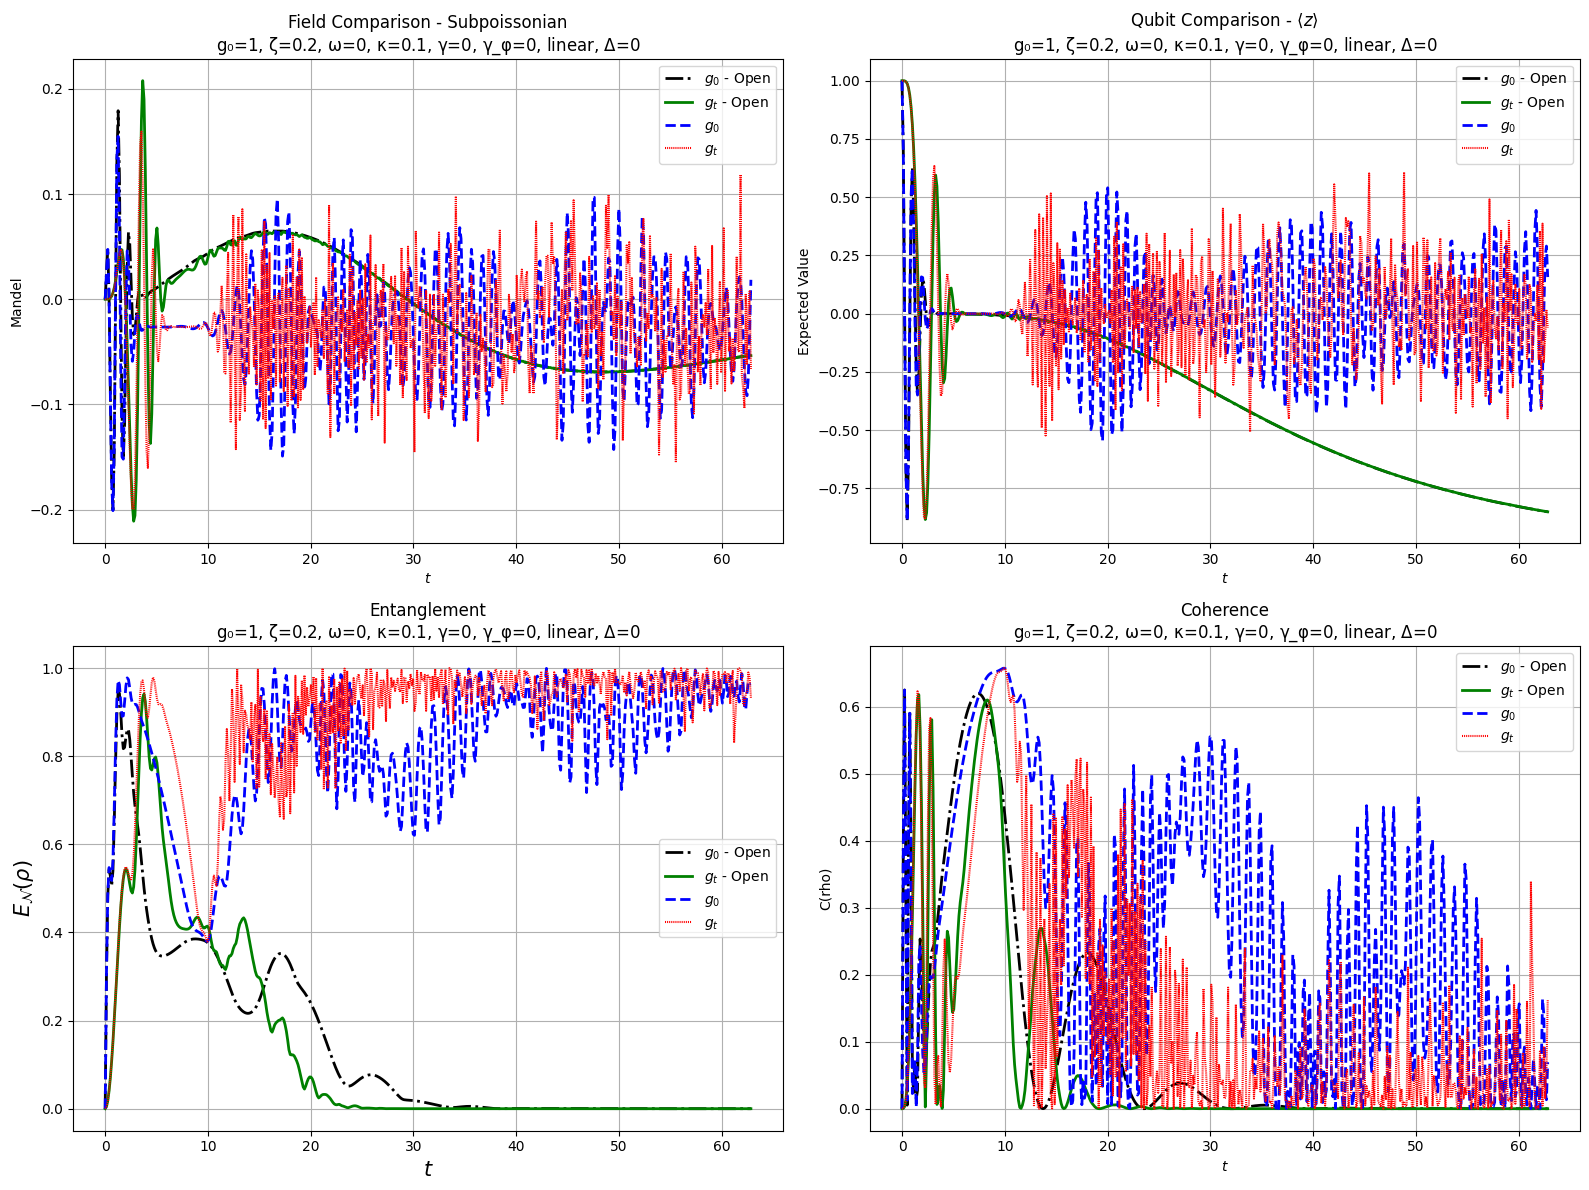
\includegraphics[width=1\linewidth]{images/grid_cavity_6.png}
    \caption{Results for $g_0=1,\,\zeta=0.2,\,\omega=0, \, \kappa=0.1, \,  \gamma=0, \, \gamma_{\phi_0}=0, \, \Delta=0$.}
    \label{fig:grid_cavity_6}
\end{figure}

\subsection{$g_0=1,\,\zeta=0.2,\,\omega=0, \, \kappa=0.05, \,  \gamma=0, \, \gamma_{\phi_0}=0, \, \Delta=0$}

\begin{figure}
    \centering
    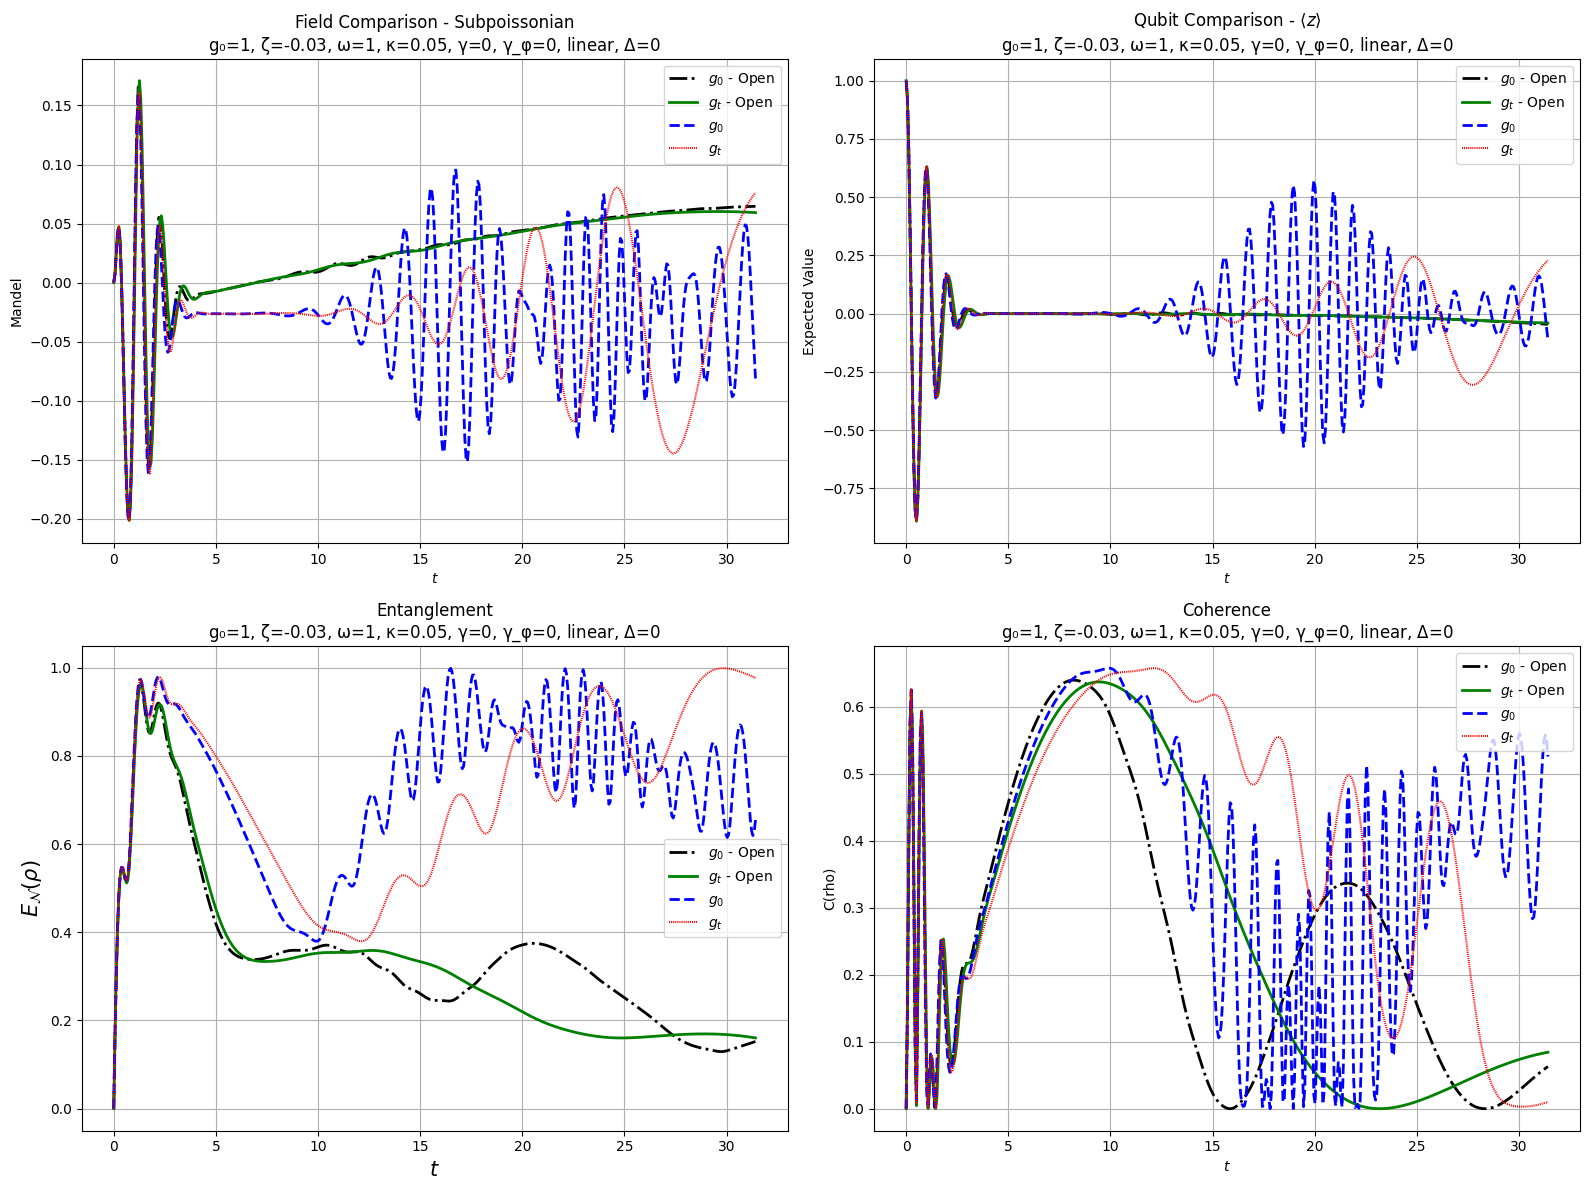
\includegraphics[width=1\linewidth]{images/grid_cavity_7.png}
    \caption{$g_0=1,\,\zeta=-0.03,\,\omega=1, \, \kappa=0.05, \,  \gamma=0, \, \gamma_{\phi_0}=0, \, \Delta=0$}
    \label{fig:grid_cavity_7}
\end{figure}

\subsection{$g_0=1,\,\zeta=0.2,\,\omega=0, \, \kappa=0.05, \,  \gamma=0.05, \, \gamma_{\phi_0}=0, \, \Delta=0$}

\begin{figure}
    \centering
    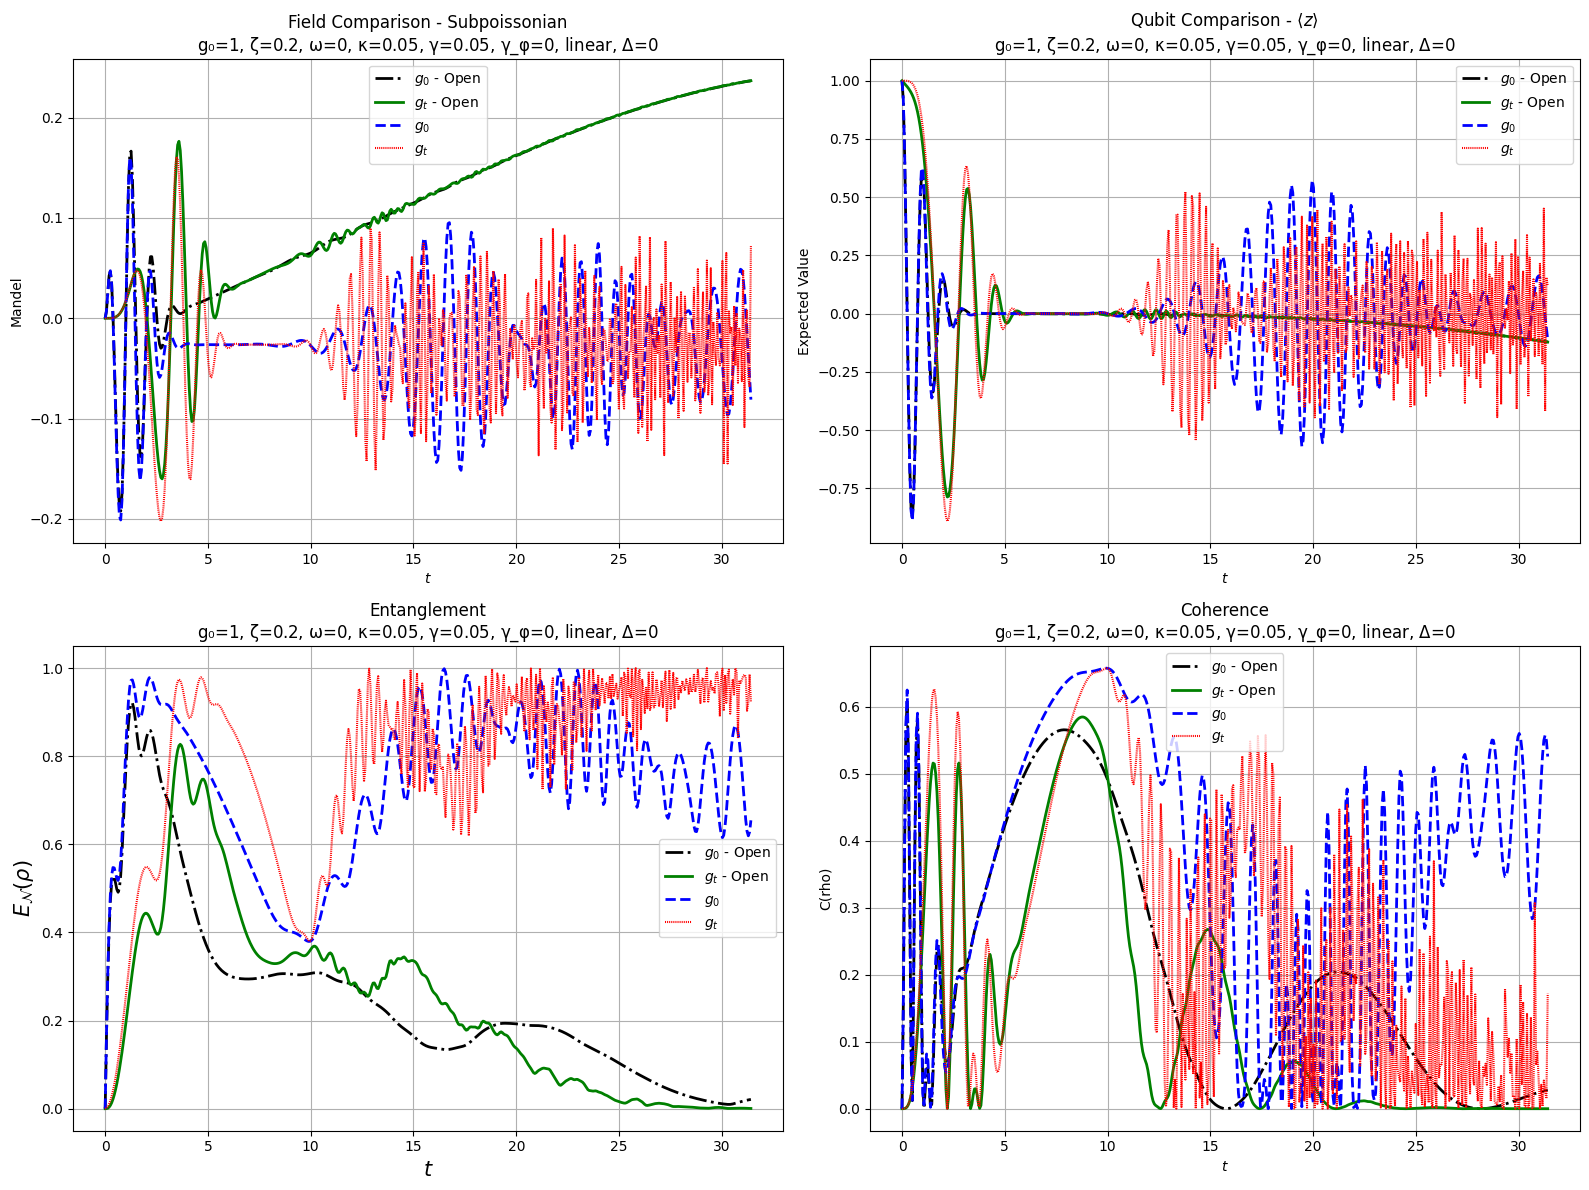
\includegraphics[width=1\linewidth]{images/grid_cavity_8.png}
    \caption{$g_0=1,\,\zeta=0.2,\,\omega=0, \, \kappa=0.05, \,  \gamma=0.05, \, \gamma_{\phi_0}=0, \, \Delta=0$}
    \label{fig:grid_cavity_8}
\end{figure}

\subsection{$g_0=1,\,\zeta=0.2,\,\omega=0, \, \kappa=0.05, \,  \gamma=0, \, \gamma_{\phi_0}=0.05, \, \Delta=0$}

\begin{figure}
    \centering
    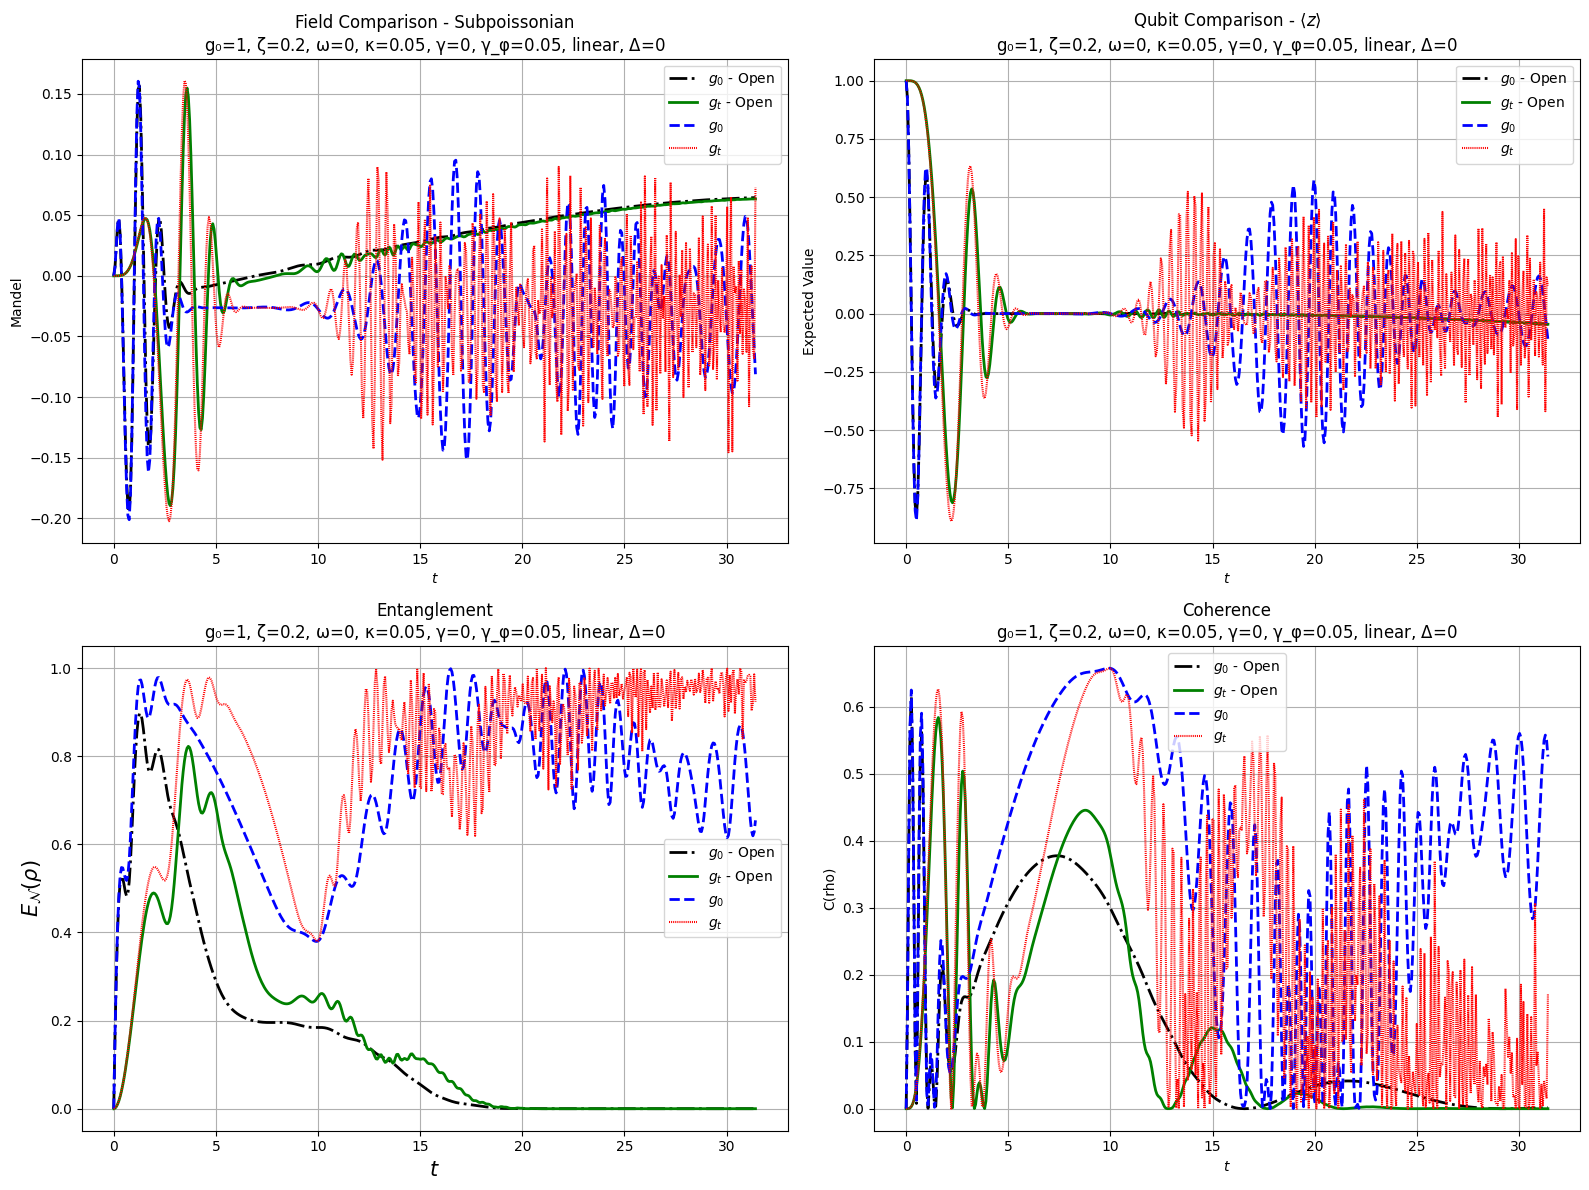
\includegraphics[width=1\linewidth]{images/grid_cavity_9.png}
    \caption{$g_0=1,\,\zeta=0.2,\,\omega=0, \, \kappa=0.05, \,  \gamma=0, \, \gamma_{\phi_0}=0.05, \, \Delta=0$}
    \label{fig:grid_cavity_9}
\end{figure}

\subsection{$g_0=1,\,\zeta=0.2,\,\omega=0, \, \kappa=0.05, \,  \gamma=0.05, \, \gamma_{\phi_0}=0.05, \, \Delta=0$}
All kinds of dissipation.
\begin{figure}
    \centering
    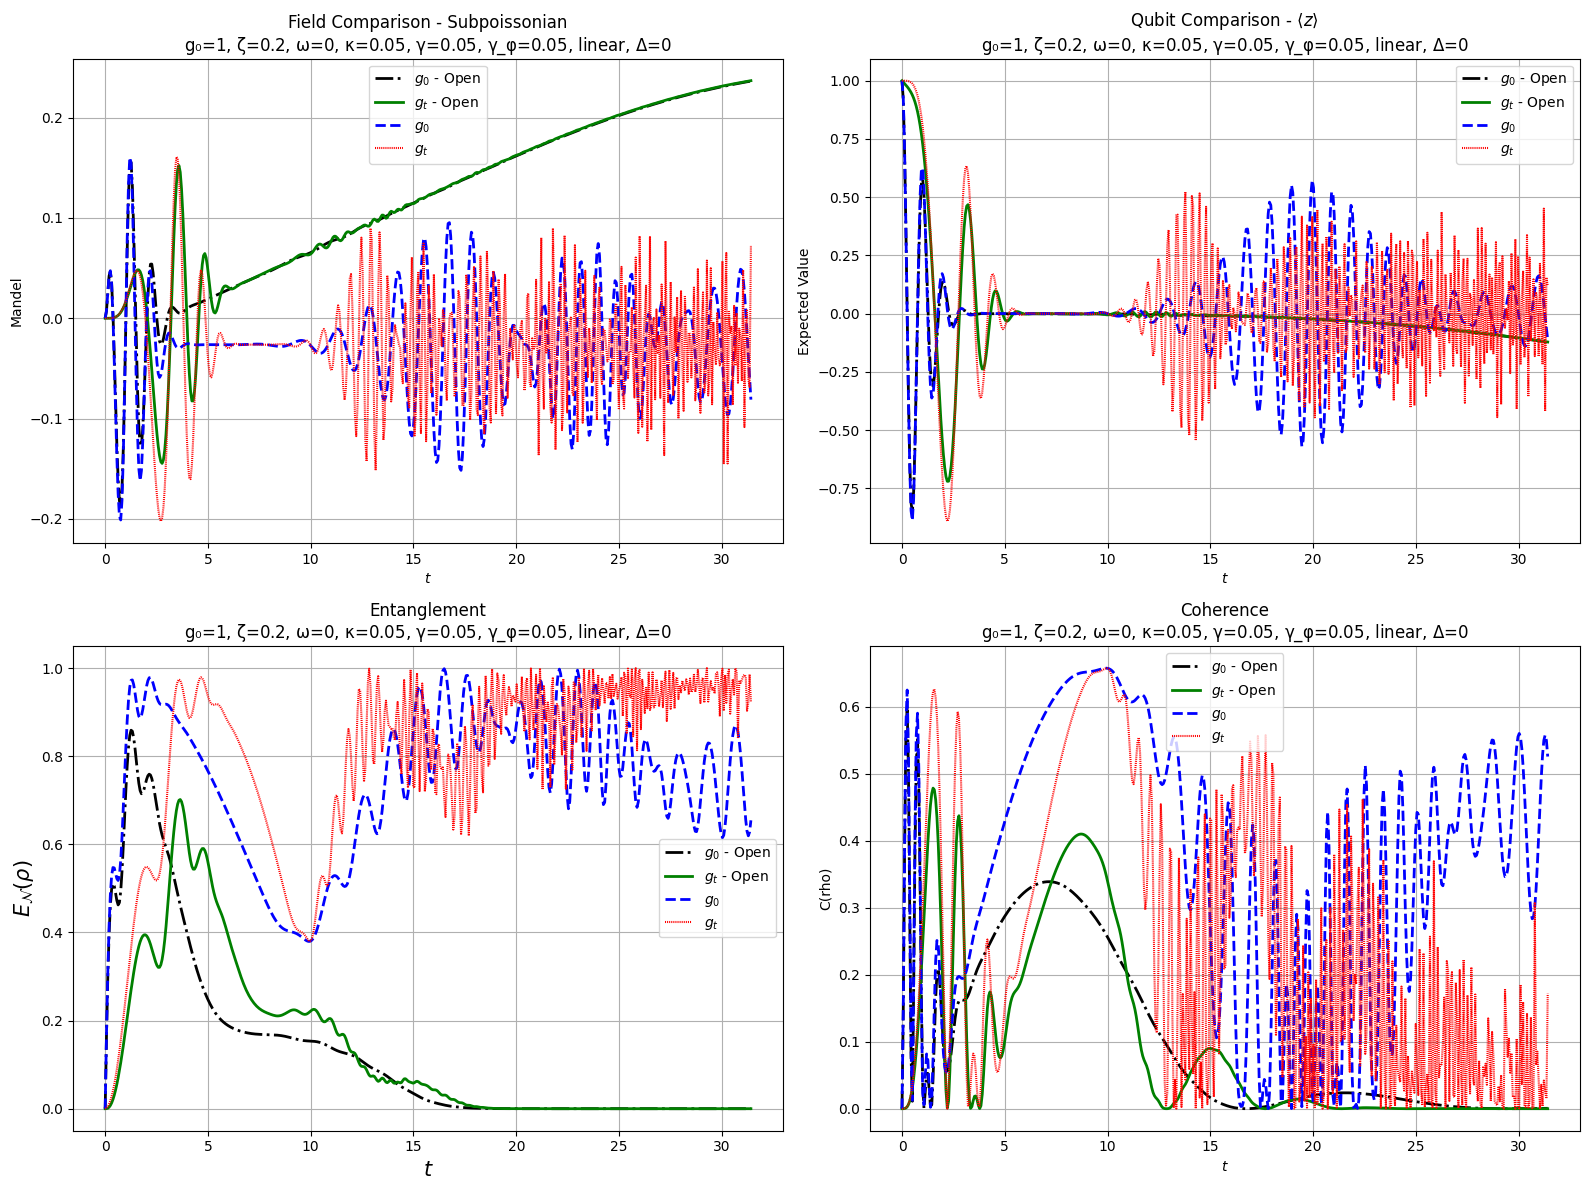
\includegraphics[width=1\linewidth]{images/grid_cavity_10.png}
    \caption{$g_0=1,\,\zeta=0.2,\,\omega=0, \, \kappa=0.05, \,  \gamma=0.05, \, \gamma_{\phi_0}=0.05, \, \Delta=0$}
    \label{fig:grid_cavity_10}
\end{figure}

\subsection{$g_0=1,\,\zeta=0.2,\,\omega=0, \, \kappa=0, \,  \gamma=0.05, \, \gamma_{\phi_0}=0.05, \, \Delta=0$}
Only atomic dissipation and linear sweep.

\begin{figure}
    \centering
    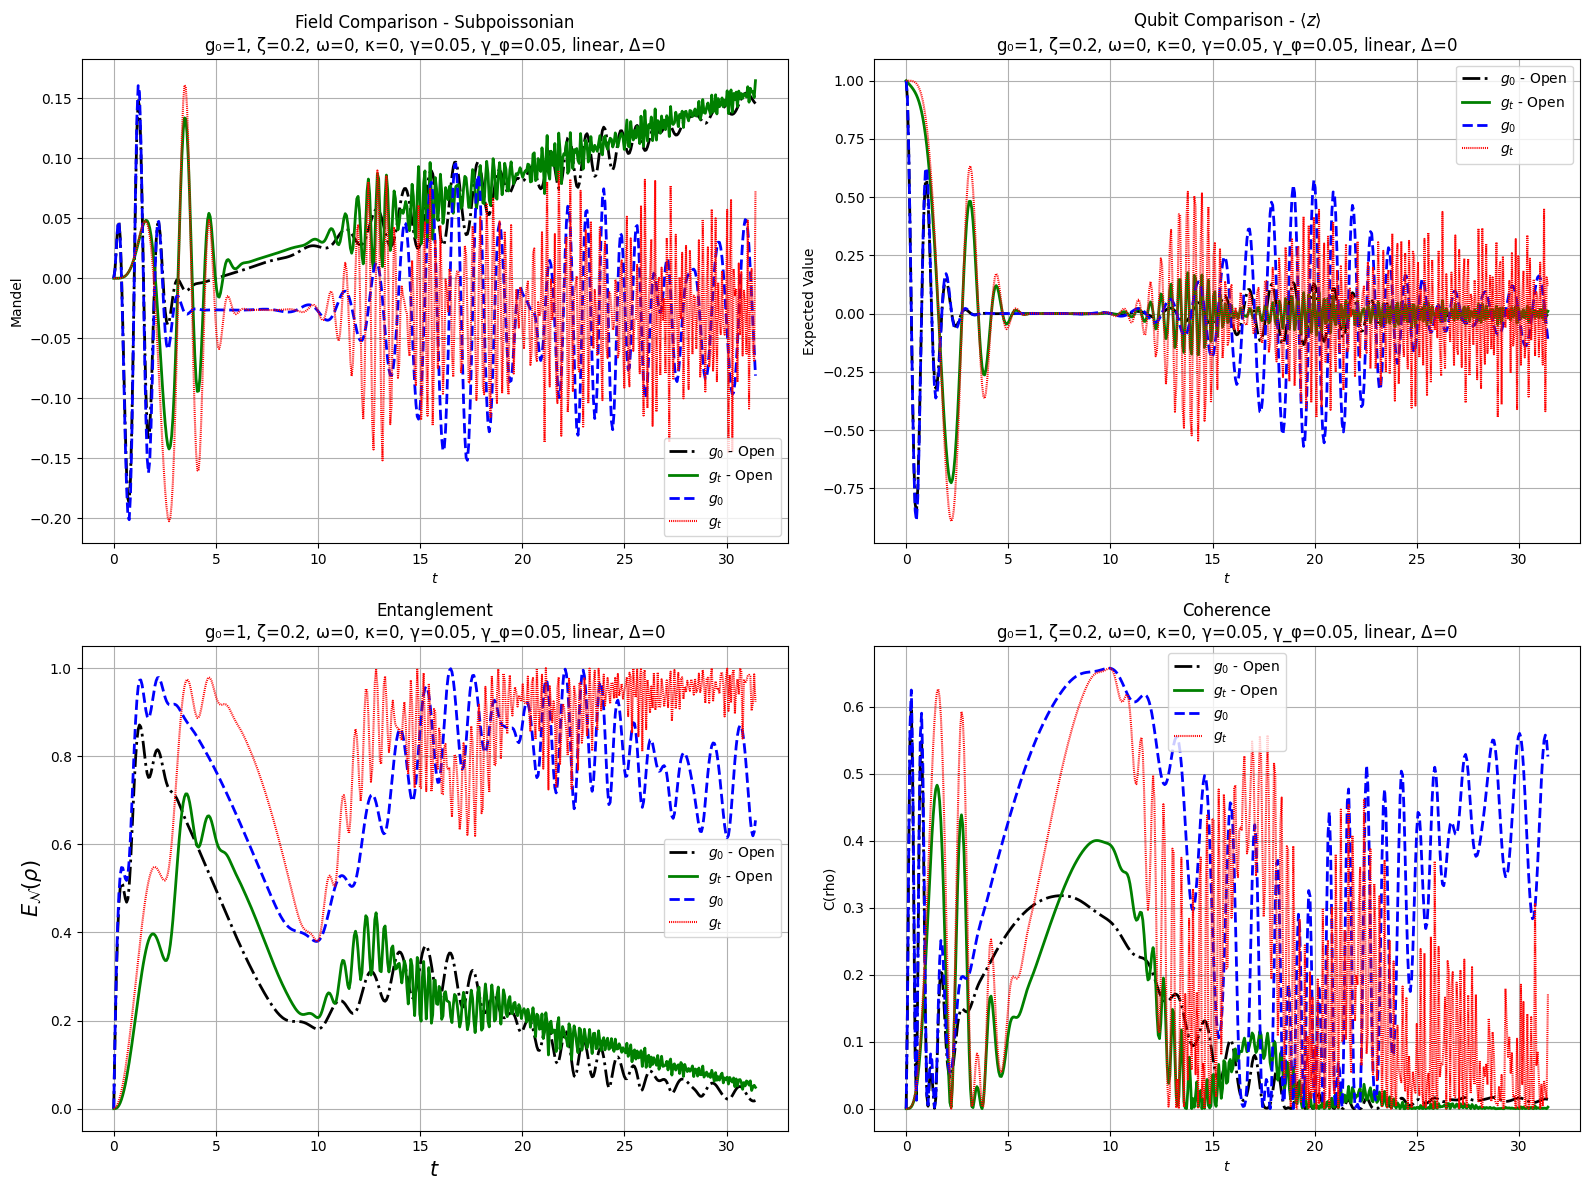
\includegraphics[width=1\linewidth]{images/grid_cavity_linqu.png}
    \caption{$g_0=1,\,\zeta=0.2,\,\omega=0, \, \kappa=0, \,  \gamma=0.05, \, \gamma_{\phi_0}=0.05, \, \Delta=0$}
    \label{fig:grid_cavity_linqu}
\end{figure}

\section{Exponential coupling}

Now, we consider a modulation of the type 
\begin{equation}
    g(t)=g_0 [\exp\left(\zeta t+\phi\right)+\omega].
\end{equation}

\subsection{$g_0=1,\,\zeta=0.062,\,\omega=-1,\,\phi=0 \, \kappa=0.05, \,  \gamma=0, \, \gamma_{\phi_0}=0$}

Here,
\begin{equation}
    \zeta=\frac{\log(g(10\pi)+\omega)}{10\pi}\approx0.062\text{ for }g(10\pi)\approx6
\end{equation}

Interestingly, the entanglement plot presents a certain advantage with this coupling. 

\begin{figure}
    \centering
    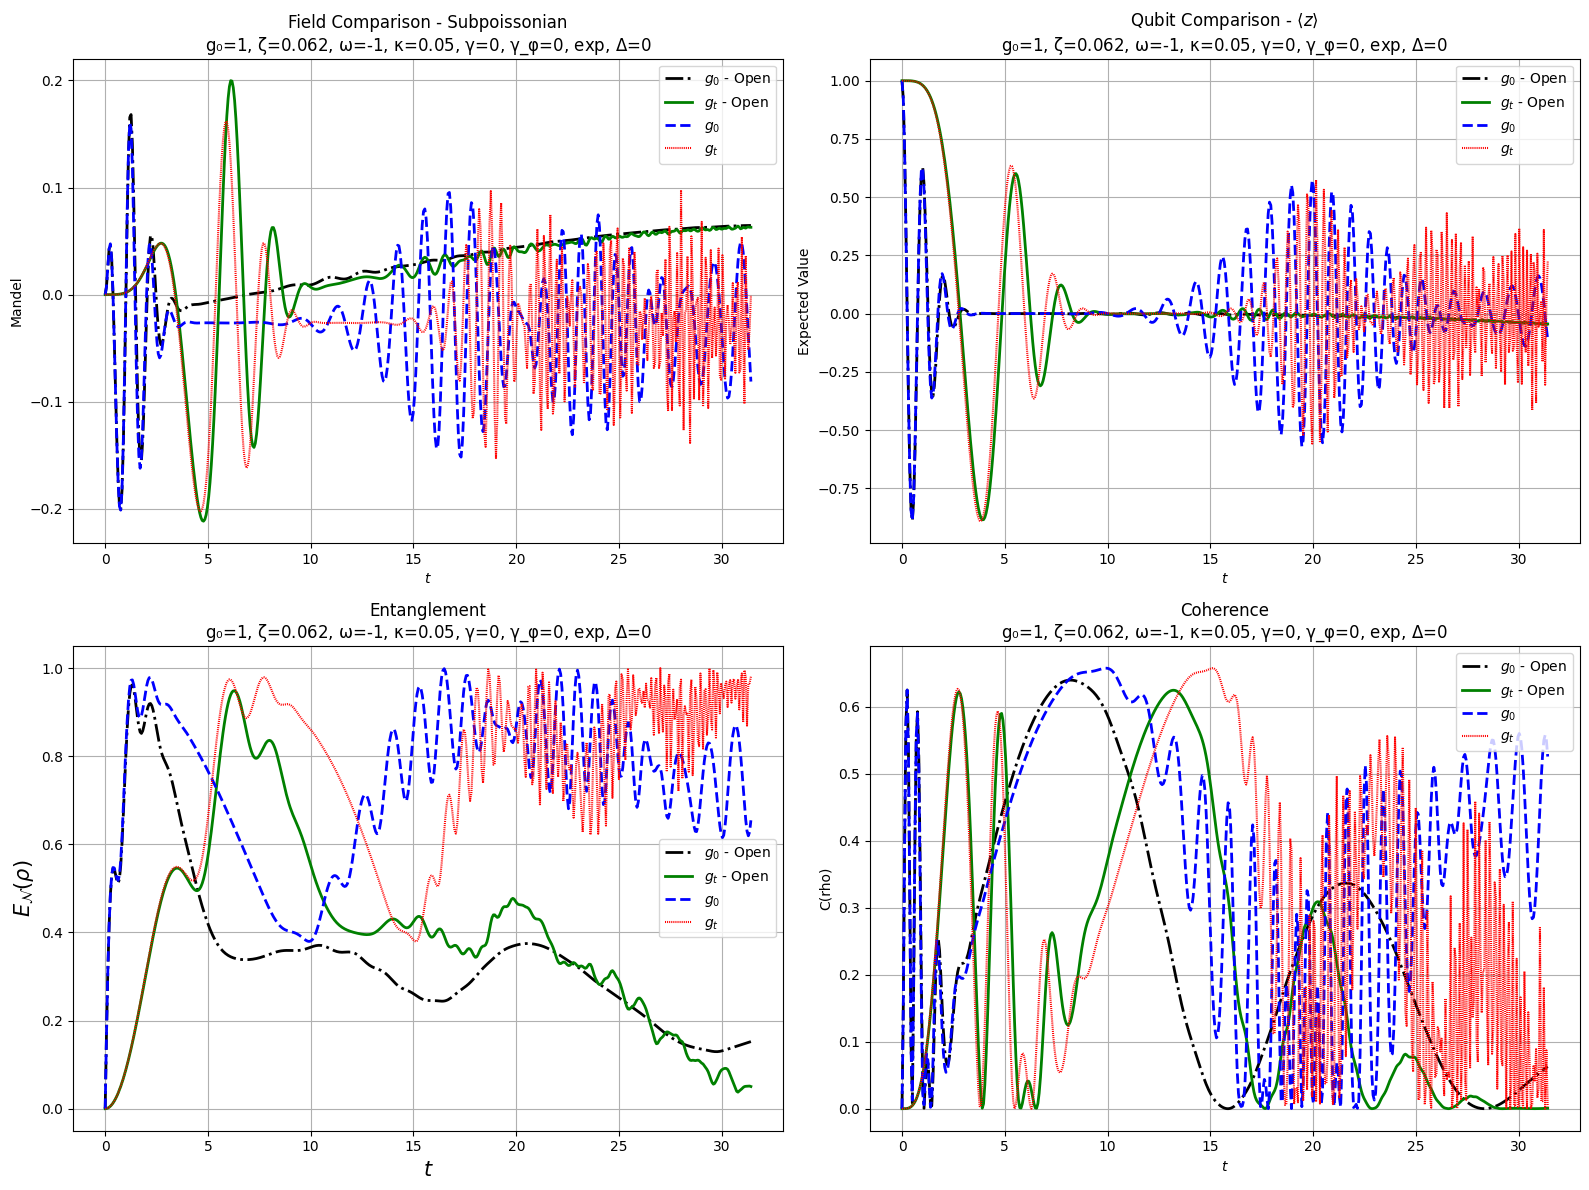
\includegraphics[width=1\linewidth]{images/grid_cavity_11.png}
    \caption{$g_0=1,\,\zeta=0.062,\,\omega=-1,\,\phi=0 \, \kappa=0.05, \,  \gamma=0, \, \gamma_{\phi_0}=0$.}
    \label{fig:placeholder}
\end{figure}

\subsection{$g_0=1,\,\zeta=-0.15,\,\omega=0,\,\phi=0, \, \kappa=0.05, \,  \gamma=0, \, \gamma_{\phi_0}=0$}

Here,
\begin{equation}
    \zeta=\frac{\log(g(10\pi)+\omega)}{10\pi}\approx-0.15\text{ for }g(10\pi)\approx0
\end{equation}

\begin{figure}
    \centering
    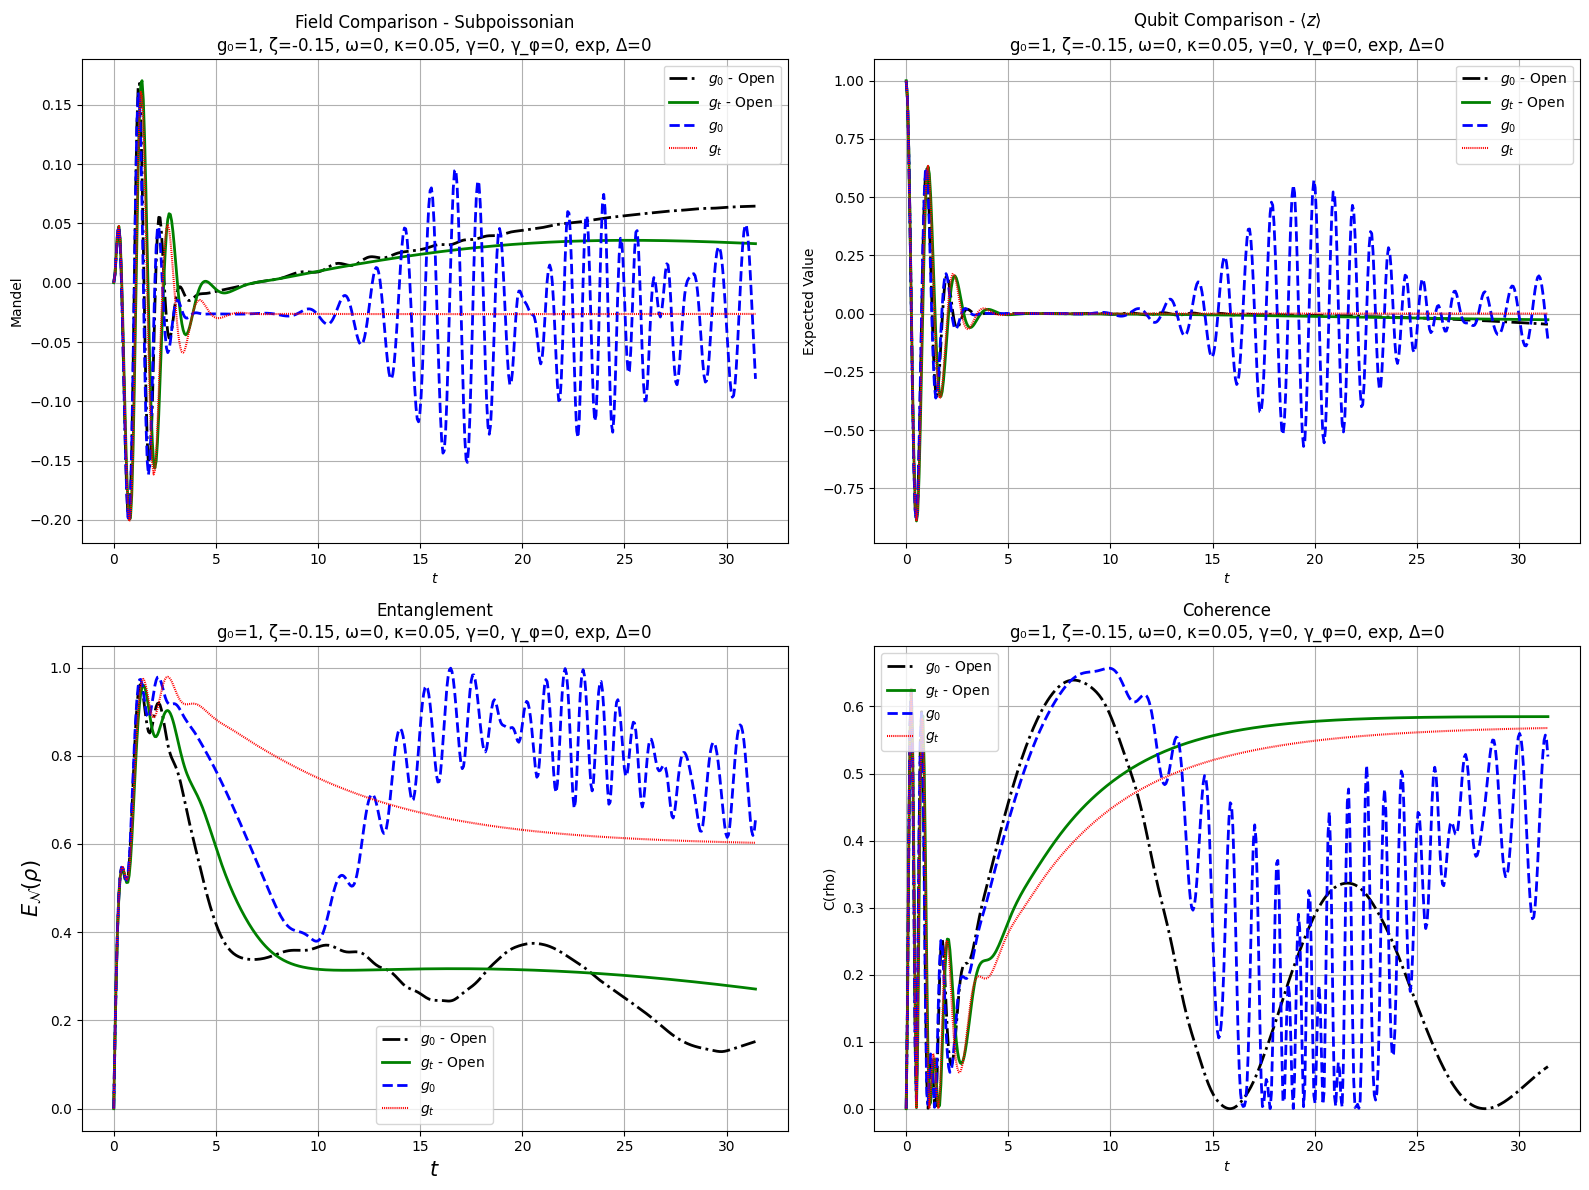
\includegraphics[width=1\linewidth]{images/grid_cavity_12.png}
    \caption{$g_0=1,\,\zeta=-0.15,\,\omega=0,\,\phi=0, \, \kappa=0.05, \,  \gamma=0, \, \gamma_{\phi_0}=0$}
    \label{fig:grid_cavity_12}
\end{figure}

\subsection{$g_0=1,\,\zeta=0.062,\,\omega=-1,\,\phi=0 \, \kappa=0, \,  \gamma=0.05, \, \gamma_{\phi_0}=0$}
Only decoherence.

\begin{figure}
    \centering
    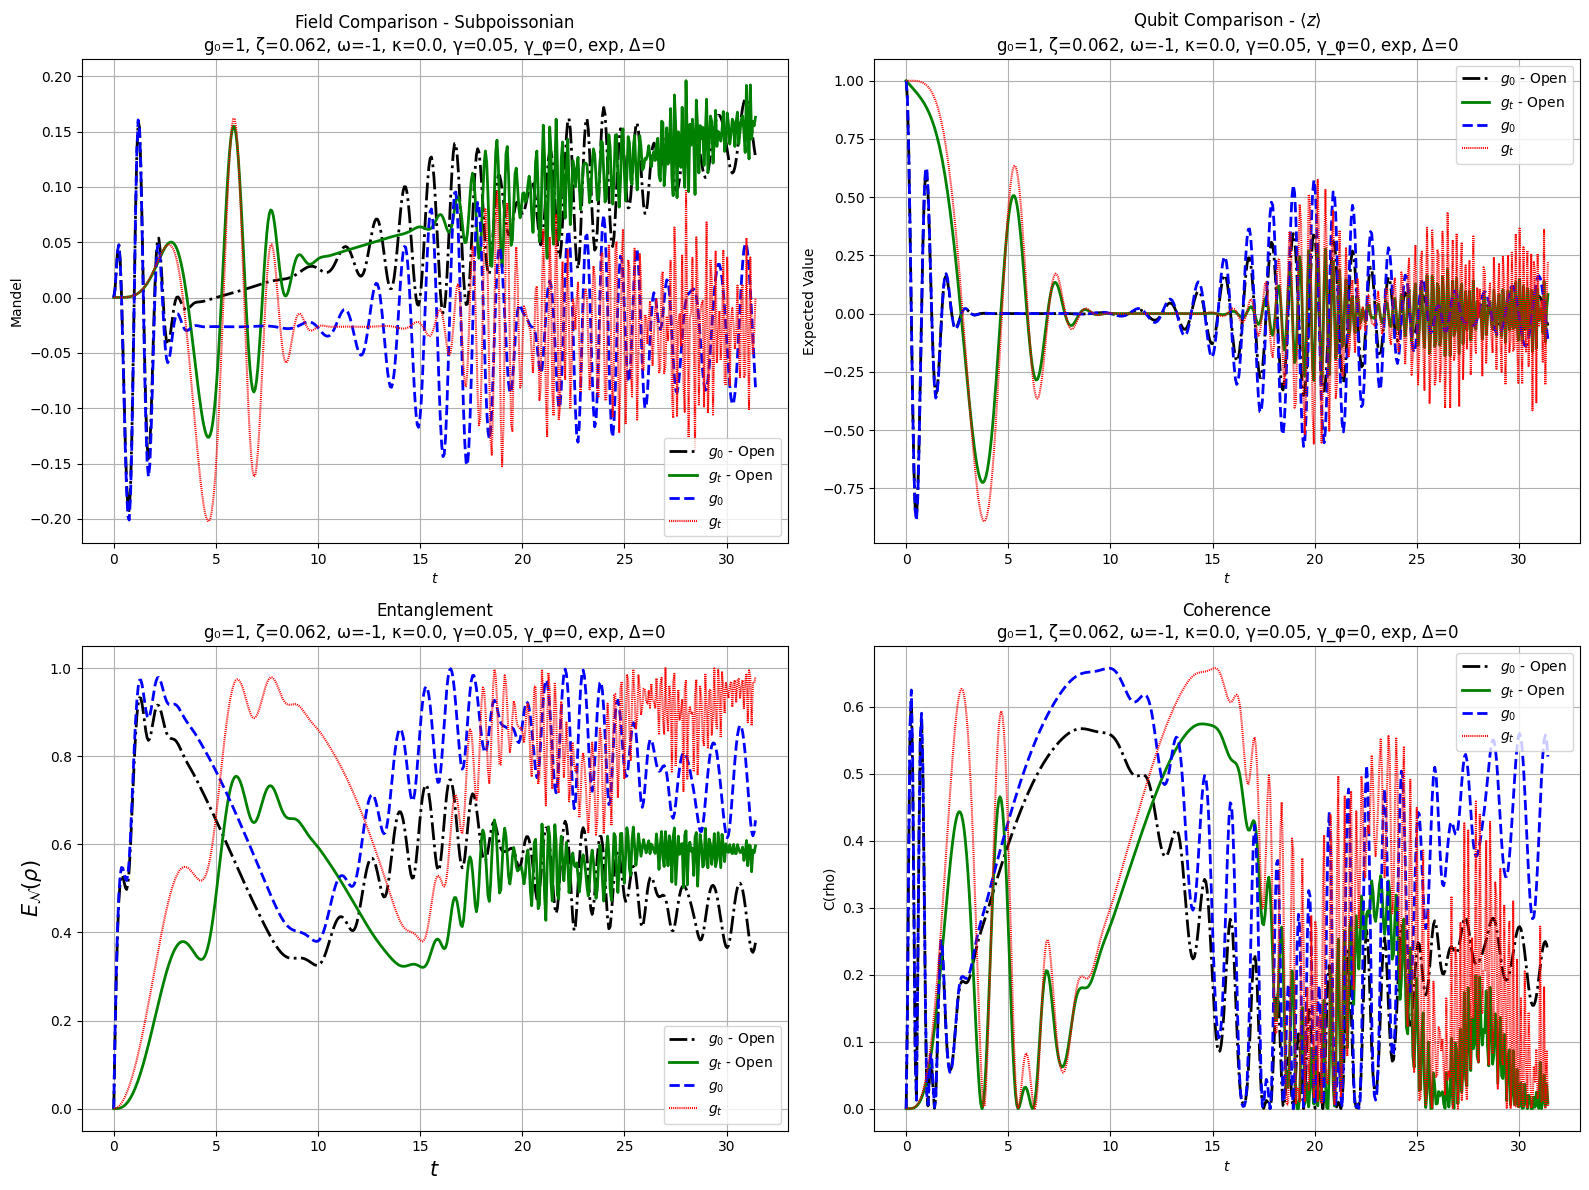
\includegraphics[width=1\linewidth]{images/grid_cavity_13.png}
    \caption{$g_0=1,\,\zeta=0.062,\,\omega=-1,\,\phi=0 \, \kappa=0, \,  \gamma=0.05, \, \gamma_{\phi_0}=0$}
    \label{fig:grid_cavity_13}
\end{figure}

\subsection{$g_0=1,\,\zeta=0.062,\,\omega=-1,\,\phi=0 \, \kappa=0, \,  \gamma=0, \, \gamma_{\phi_0}=0.05$}
Only dephasing.

\begin{figure}
    \centering
    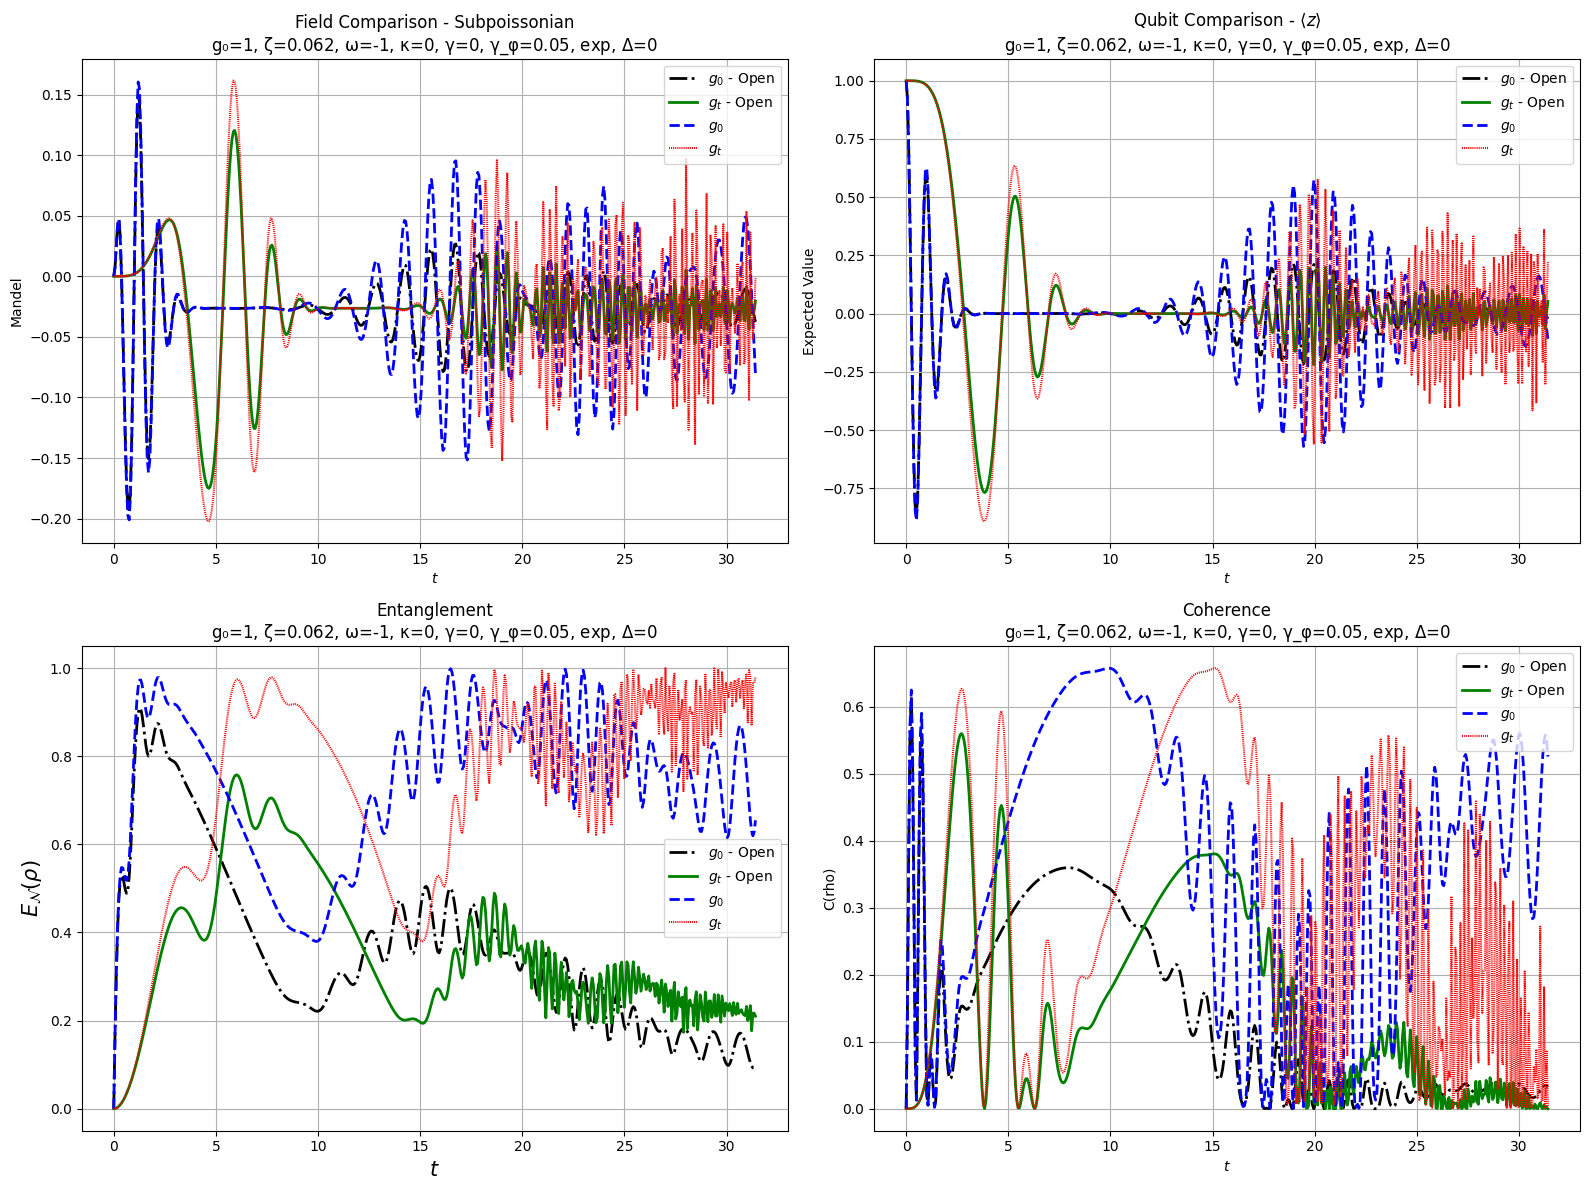
\includegraphics[width=1\linewidth]{images/grid_cavity_14.png}
    \caption{$g_0=1,\,\zeta=0.062,\,\omega=-1,\,\phi=0 \, \kappa=0, \,  \gamma=0, \, \gamma_{\phi_0}=0.05$}
    \label{fig:grid_cavity_14}
\end{figure}

\subsection{$g_0=1,\,\zeta=0.062,\,\omega=-1,\,\phi=0 \, \kappa=0, \,  \gamma=0.05, \, \gamma_{\phi_0}=0.05$}
Both kinds of qubit dissipation.

\begin{figure}
    \centering
    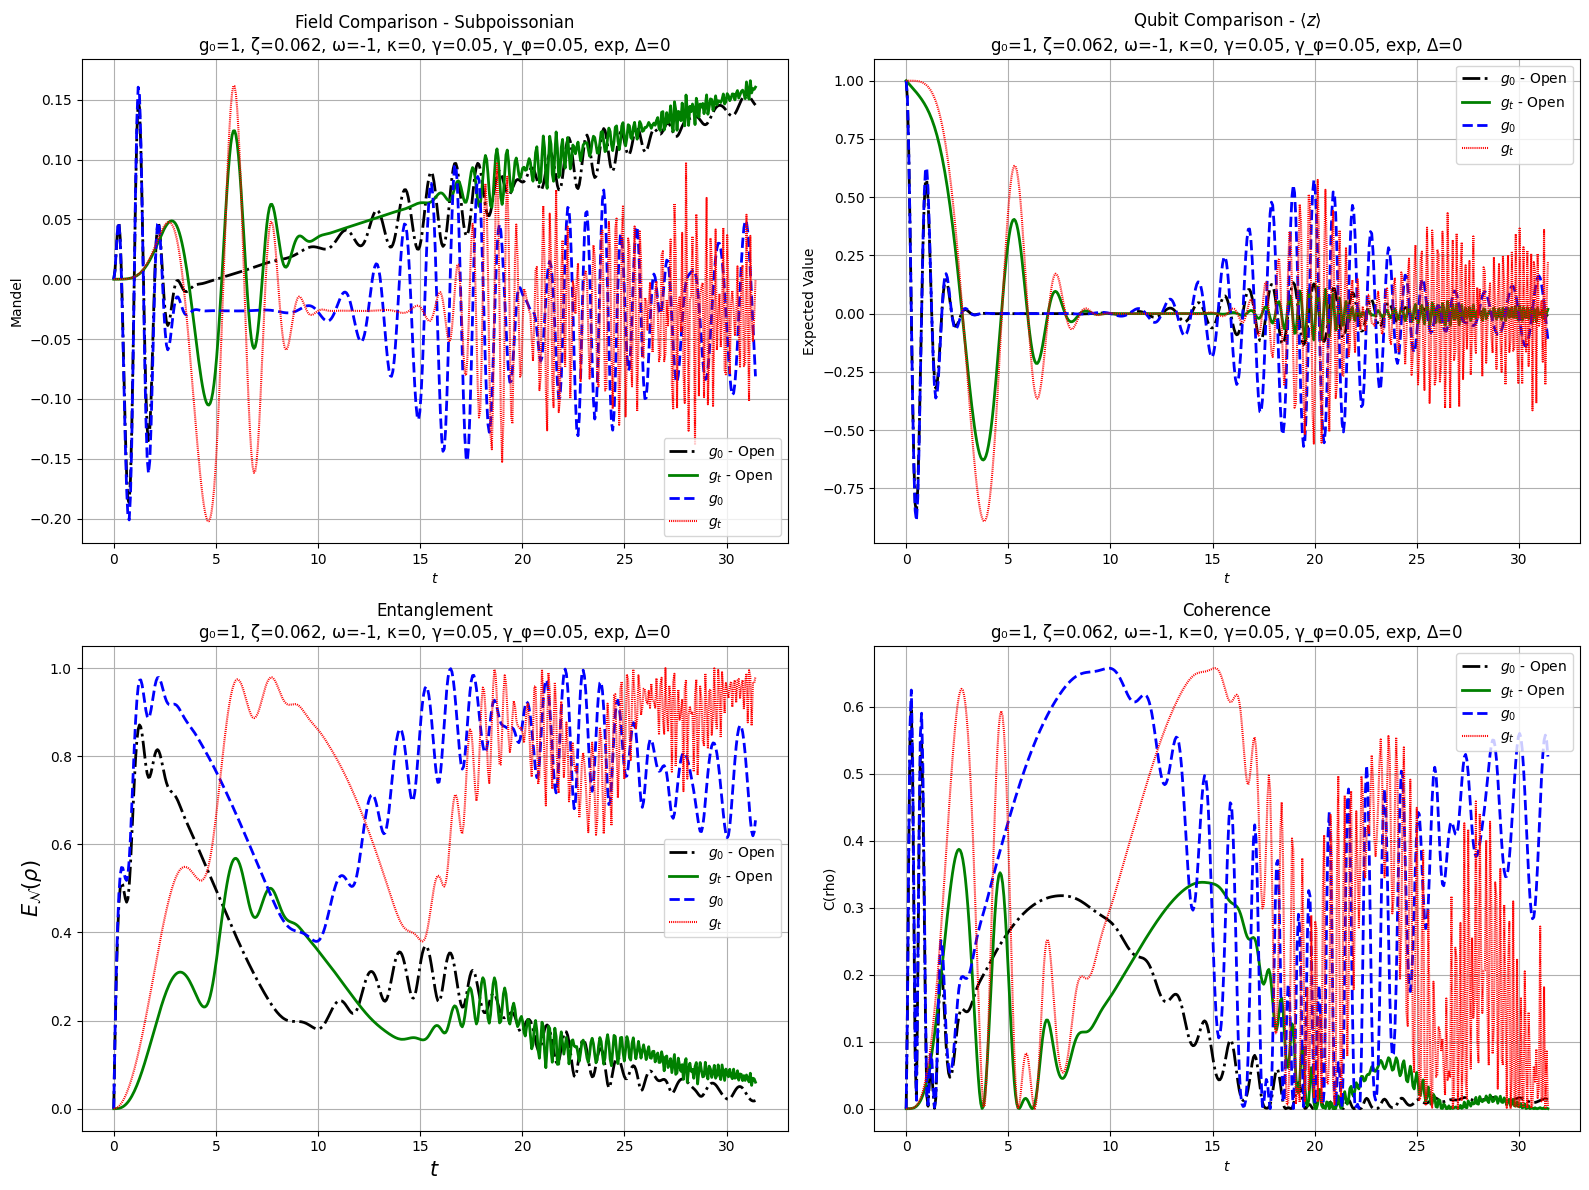
\includegraphics[width=1\linewidth]{images/grid_cavity_15.png}
    \caption{$g_0=1,\,\zeta=0.062,\,\omega=-1,\,\phi=0 \, \kappa=0, \,  \gamma=0.05, \, \gamma_{\phi_0}=0.05$}
    \label{fig:grid_cavity_15}
\end{figure}


\section{Trigonometric coupling}
To assess the advantages introduced by the time-dependent couplings 
$g_s(t)=g_0 \sin(\omega t)$ and $g_c(t)=g_0 \cos(\omega t)$, we consider the initial product state
\begin{equation}
    \ket{\psi_0} = \ket{+}\ket{\alpha},
\end{equation}
where $\ket{+} = (\ket{0}+\ket{1})/\sqrt{2}$ is the eigenstate of the Pauli operator $\sigma_x$, and
\begin{equation}
    \ket{\alpha} = e^{-|\alpha|^2/2} 
    \sum_{n=0}^{\infty} \frac{\alpha^n}{\sqrt{n!}} \ket{n}
\end{equation}
is a coherent state with $|\alpha|^2 = \langle n \rangle = 10$.
The qubit state $\ket{+}$ exhibits maximal coherence $C(\rho^Q)=\ln 2$, and is therefore well suited to probe how time-dependent coupling modulations influence the preservation of nonclassical resources.
Figure~\ref{fig:c_trigonometric_a} displays the time evolution of $C(\rho^Q)$ for $\omega = 1$, $g_0 = 1$, $\kappa = 0.1$, and $\gamma = 0.01$, comparing the performance of the two modulated couplings with that of the constant interaction. 
Both $g_s(t)$ and $g_c(t)$ extend the coherence lifetime relative to the static case, demonstrating that temporal modulation can mitigate the degradation of quantum resources.

To quantify how this enhancement depends on the modulation frequency, we introduce the coherence-limit time $\tau$, defined as the first time at which $C(\rho^Q)<10^{-5}$. 
The dependence of $\tau$ on $\omega$, shown in Fig.~\ref{fig:c_trigonometric_b}, reveals that both time-dependent couplings consistently outperform the static interaction. 
Furthermore, $g_s(t)$ yields systematically longer coherence times than $g_c(t)$ across all frequencies investigated. 
For both modulations, $\tau$ increases sharply for $\omega \lesssim 1$, followed by a slower growth in the high-frequency regime $\omega > 1$.

The improved coherence observed under modulated interactions can be attributed to the dynamical control imparted by the oscillatory coupling. 
Because the qubit--field coupling is not continuously active, the qubit experiences a periodically suppressed interaction with the dissipative environment. 
For moderate frequencies ($\omega \leq 1$), this mechanism resembles a dynamical-decoupling protocol: the rapid modulation averages out the noise and thereby suppresses decoherence. 
At higher frequencies, the system enters a regime in which the coupling oscillates too rapidly for the cavity losses to respond, leading to the saturation observed in $\tau(\omega)$. 
Among the two modulations, the sine profile $g_s(t)$ achieves the longest coherence times because it begins with vanishing coupling strength, thereby minimizing the initial dissipation rate and prolonging the survival of coherence.



\begin{figure}[ht]
    \centering
    % --- Subfigura (a) ---
    \begin{subfigure}{0.48\linewidth}
        \centering
        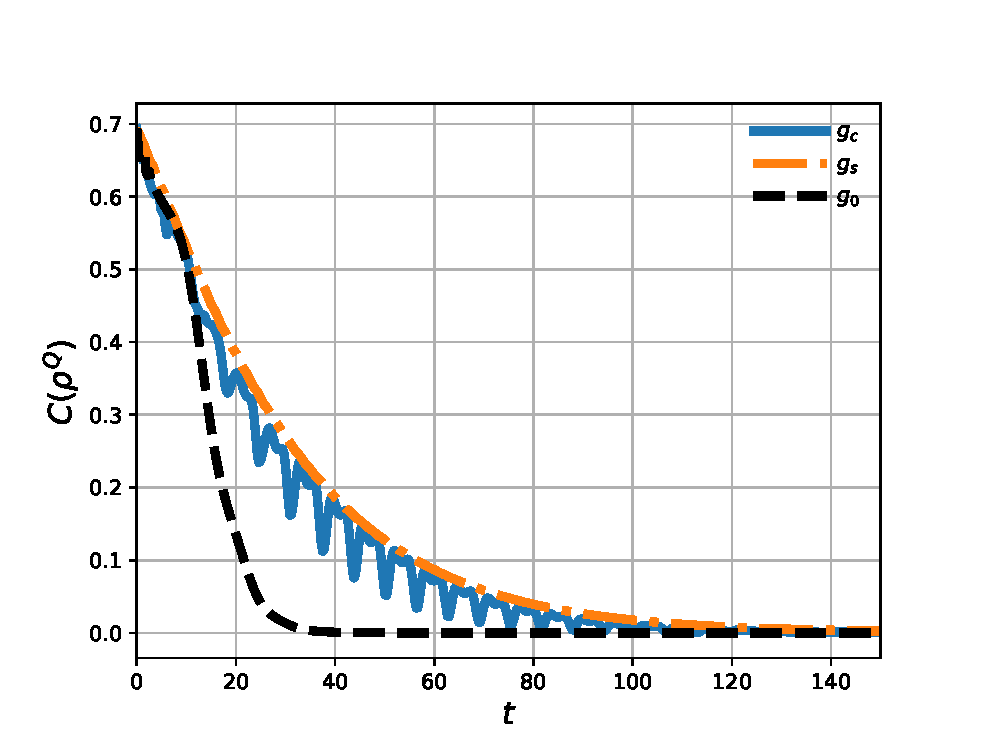
\includegraphics[width=\linewidth]{images/trigonometric.eps}
        \caption{}
        \label{fig:c_trigonometric_a}
    \end{subfigure}
    \hfill
    % --- Subfigura (b) ---
    \begin{subfigure}{0.48\linewidth}
        \centering
        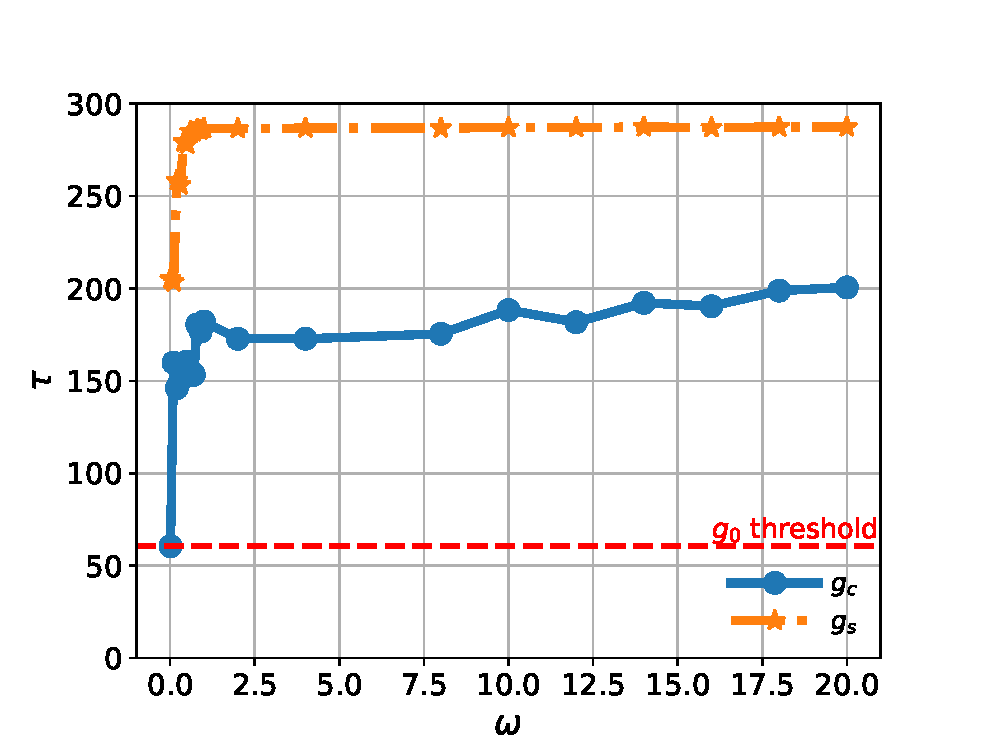
\includegraphics[width=\linewidth]{images/trigonometric_tau.eps}
        \caption{}
        \label{fig:c_trigonometric_b}
    \end{subfigure}

    \caption{
    (a) Time evolution of the qubit coherence $C(\rho^Q)$ for the initial state 
    $\ket{\psi_0}=\ket{+}\ket{\alpha}$ under three coupling types: the cosine modulation 
    $g_c(t)=g_0\cos(\omega t)$, the sine modulation $g_s(t)=g_0\sin(\omega t)$, and the 
    constant interaction $g_0$. With $\omega=1$, $g_0=1$, $\kappa=0.1$, and $\gamma=0.01$. 
    (b) Coherence limit time $\tau$ as a 
    function of the driving frequency $\omega$.
}

    \label{fig:c_trigonometric_combined}
\end{figure}



\section{Detuning effects}
Detuning may help with  entanglement and atomic population dynamics resilience?
\begin{figure}
    \centering
    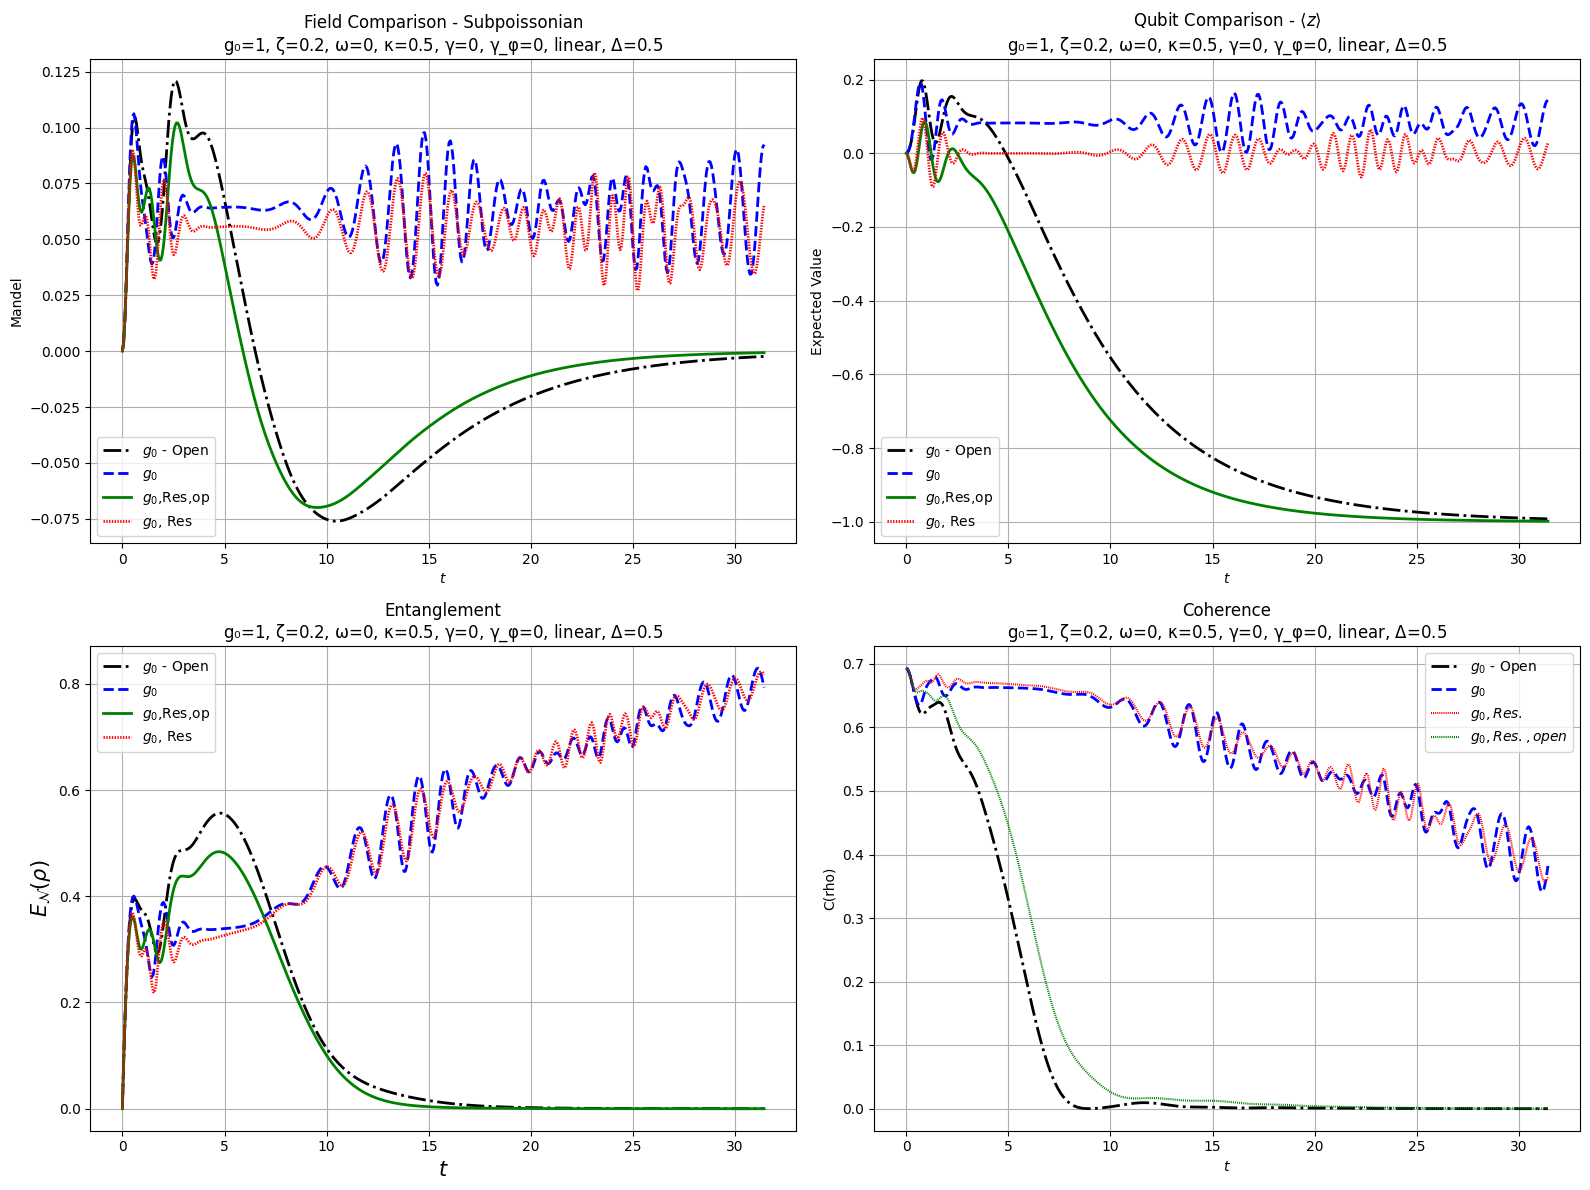
\includegraphics[width=1\linewidth]{images/grid_cavity_16.png}
    \caption{$g_0=1,\,\phi=0 \, \kappa=0.05 \,  \gamma=0, \, \gamma_{\phi_0}=0,\Delta=0.5$}
    \label{fig:grid_cavity_16}
\end{figure}

\section{Comparing with Puri1986}
In 1986, Puri and Agarwal published a work studying the collapse and revival phenomena considering cavity dissipation \cite{Puri1986}.
In that work, they actually plotted the probability of the atom being excited, but we can extract the general behavior from there. 
Here, we employ the same dissipation factors. 
We changed the initial average photon number to $\langle\hat{n}(0)\rangle=5$ and choose the exponential time modulation with slow start. 
In Figs. \ref{fig:puri1} and \ref{fig:puri2}, we see that the time-dependent coupling results in a revival with bigger amplitudes -- although with delayed start.
In Fig. \ref{fig:puri3}, we see that the exponential modulation has a bigger influence on the average photon number at the start.

\begin{figure}
    \centering
    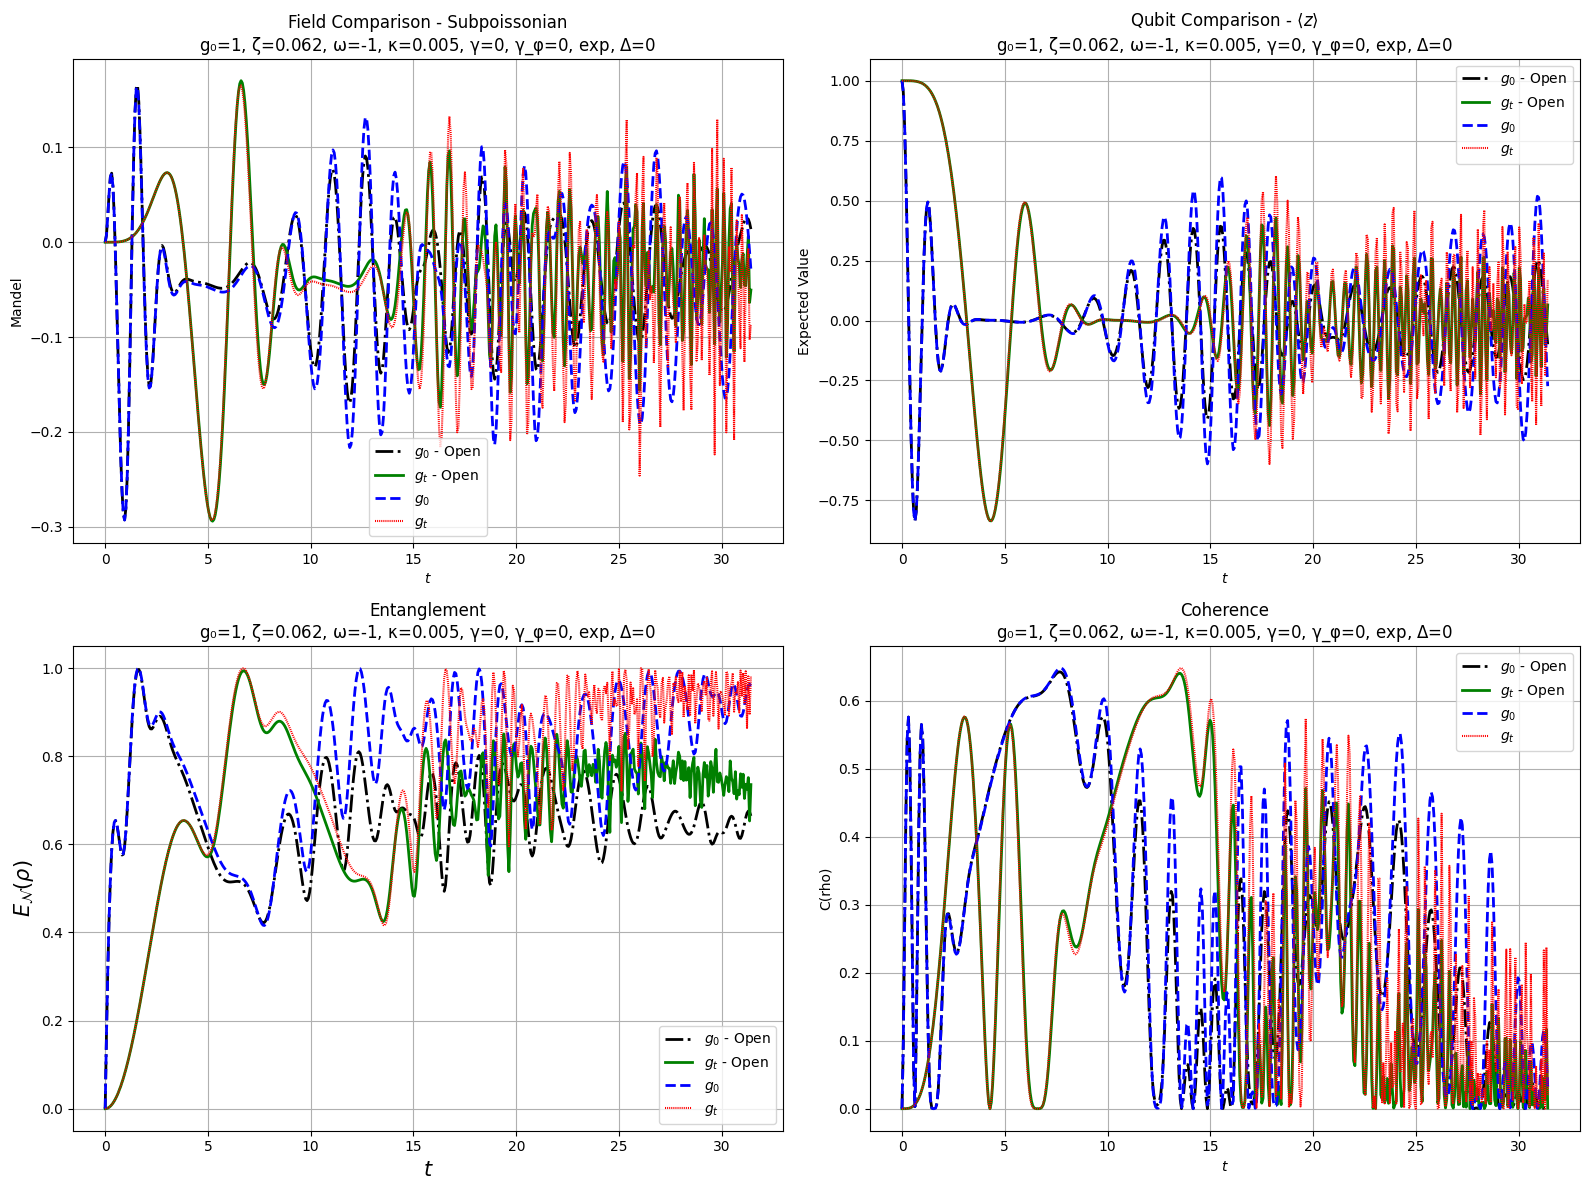
\includegraphics[width=1\linewidth]{images/puri1.png}
    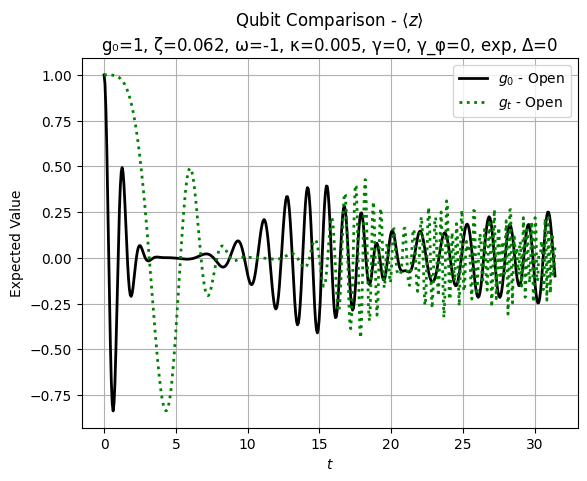
\includegraphics[width=0.35\linewidth]{images/puri1_only_pop.png}
    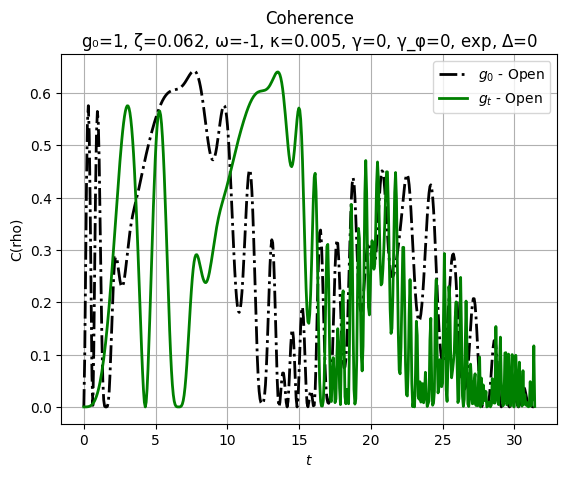
\includegraphics[width=0.35\linewidth]{images/puri1_only_coh.png}
    \caption{$g_0=1,\,\phi=0 \, \kappa=0.005 \,  \gamma=0, \, \gamma_{\phi_0}=0,\Delta=0.5$ and initial average photon number $\langle\hat{n}(0)\rangle=5$.
    We obtain a revivel with bigger amplitude.}
    \label{fig:puri1}
\end{figure}

\begin{figure}
    \centering
    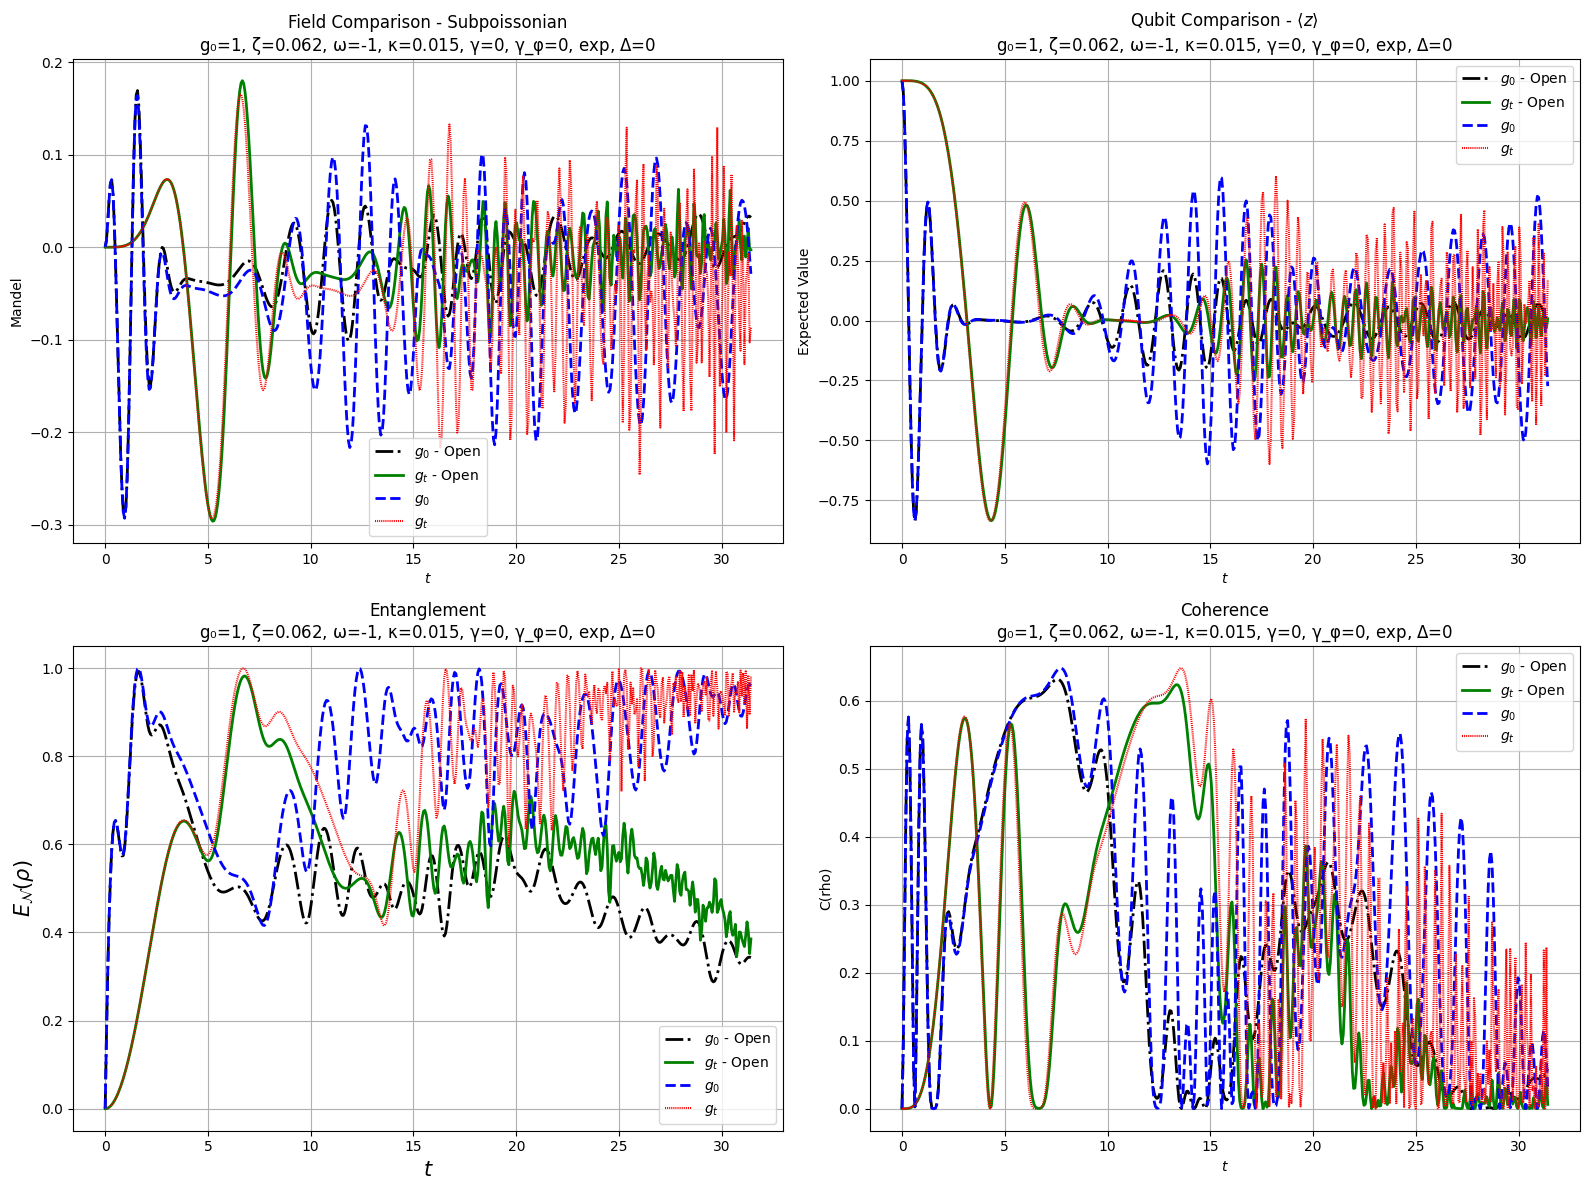
\includegraphics[width=0.75\linewidth]{images/puri2.png}
    \caption{$g_0=1,\,\phi=0 \, \kappa=0.005 \,  \gamma=0, \, \gamma_{\phi_0}=0,\Delta=0.5$ and initial average photon number $\langle\hat{n}(0)\rangle=5$.}
    \label{fig:puri2}
\end{figure}

\begin{figure}
    \centering
    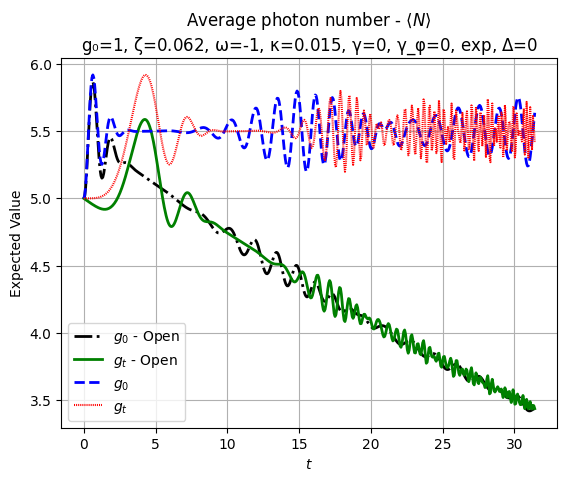
\includegraphics[width=0.5\linewidth]{images/puri3.png}
    \caption{$g_0=1,\,\phi=0 \, \kappa=0.005 \,  \gamma=0, \, \gamma_{\phi_0}=0,\Delta=0.5$ and initial average photon number $\langle\hat{n}(0)\rangle=5$.
    Here, I noticed that the time-dependent coupling overall doesn't influence the average photon number.}
    \label{fig:placeholder}
\end{figure}


\section{Ideas}
\begin{itemize}
    \item What if we start with an entangled (Bell state, for example)? Can a slow start help to protect entanglement?
    \item What about the cavity coherence? Can an sharper coupling help to protect it?
    \item Gaussian time-dependence.
\end{itemize}


\section{Time-dependent coupling as a tool for preserving quantum resources}
Baseado no que conversamos pelo whatsapp, aqui faço testes sobre a capacidade do acoplamento variável manter os recursos quânticos.


\printbibliography

\end{document}
